\documentclass{article}

%%%%%%%%%%%%%%%%%%%%%%%%% Packages %%%%%%%%%%%%%%%%%%%%%%%%%
\usepackage[utf8]{inputenc}

\usepackage{geometry}
\geometry{left = 25 mm, top = 25 mm}%pour les marges

\usepackage{amsfonts}
\usepackage{amssymb}
\usepackage{amsmath}
\usepackage{amsthm}
\usepackage{multicol}
\usepackage{diagbox}
\usepackage{hyperref}

\usepackage{xcolor} % for setting colors

\usepackage{mathtools}
\DeclarePairedDelimiter\ceil{\lceil}{\rceil}
\DeclarePairedDelimiter\floor{\lfloor}{\rfloor}

\usepackage{array}
\newcolumntype{C}{>{\(\displaystyle}c<{\)}@{}} 
\newcolumntype{L}{>{\(\displaystyle}l<{\)}@{}} 
\newcolumntype{R}{>{\(\displaystyle}r<{\)}@{}}


%%%%%%%%%%%%%%%%%%%%%%%%% Macros %%%%%%%%%%%%%%%%%%%%%%%%%
% mathbb for class of numbers macro.
\newcommand{\BB}[1]{\mathbb{#1}}

% Integral macro.
\newcommand{\intt}[4]{\displaystyle\int_{#1}^{#2}#3\;\text{d}#4}
% use :$\intt{a}{b}{f(x)}{x}$

% end line
\newcommand{\n}{\\ [6pt]}



%%%%%%%%%%%%%%%%%%%%%%%%%%%%%%%%%%%%%%%%%%%%%%%%%%%%%%%%%%%%
%%%%%%%%%%%%%%%%%%%%%%%%% Document %%%%%%%%%%%%%%%%%%%%%%%%%
\begin{document}

%%%%%%%%%%%%%%%%%%%%%%%%% Page titre %%%%%%%%%%%%%%%%%%%%%%%
\begin{titlepage}
  \centering
  
  \rule{\textwidth}{0px}
  \vspace{15mm}
  
  \Huge{Rapport} \\
  \vspace{5mm}
  \Large Bases de données \\
  IFT 2935
  
  \vspace{40mm}
  \large par \\ \vspace{3mm}
  Zakary Gaillard-Duchassin\\ \vspace{3mm}
  Mohammed Aiman Rahmani \\ \vspace{3mm}
  Samuel Argeris \\ \vspace{3mm}
  Farley Jeannis \\ \vspace{3mm}
  Mathieu Dominique Lucien Loron \\ \vspace{3mm}
  \vspace{30mm}
  présenté à \\ \vspace{3mm}
  Jihene Rezgui
  
  \vfill
  10 avril 2024 \\ \vspace{3mm}
  
\includegraphics[scale=0.55]{logo-udem.png}
\end{titlepage}
\newpage

%%%%%%%%%%%%%%%%%%%%%%%%% Contenu %%%%%%%%%%%%%%%%%%%%%%%%%%
\noindent
L'ensemble du code est disponible sur le répertoire github suivant:
\href{https://github.com/ZGaillard/projet\_session\_2935}{\color{blue}{\underline{projet\_session\_2935}}}.



\section{Modélisation}
Nous avons été assigné le sujet 11. La tâche consistait à modéliser
et implémenter une base de données qui puisse gérer l’implication des
artistes dans divers films.\n
Le cahier des charges était le suivant:\n
\textbf{Artiste}
\begin{itemize}
\item Nom, prénom, âge de l’artiste.
\item Adresse (et appartement au besoin).
\item Renseignements personnels (habitudes, sports, relations, etc.). 
\item On doit également pouvoir inscrire si l’artiste a déjà joué dans des films ou théâtres (et avec quelles compagnies). 
\item Exigences de rémunération.
\end{itemize}

D’un autre côté, on veut aussi garder des renseignements sur le casting, l’objectif du casting et le thème. On a aussi les différentes scènes du scénario, avec les exigences en termes de réalisation de scène (action, bataille, passion, discours, etc.).\n
On aura aussi besoins d’enregistrer les noms des sponsors attachés aux
films avec les montants des budgets, les détails de financement,
etc.\n


\subsection{Analyse des besoins}
\begin{itemize}
\item Les artistes peuvent avoir des habitudes et des sports.
\item Les artistes peuvent avoir des relations avec d'autres artistes.
\item Les pieces de théâtre et les films ont des scènes.
\item Les films et les pièces de théâtre ont des sponsors.
\item les pièces de théâtre et les films ont des castings.
\item Les castings ont des artistes qui y participent.
\item Les films ont des studios de production (compagnies).
\end{itemize}

  
\subsection{Modèle Entité-Association}

\begin{center}
  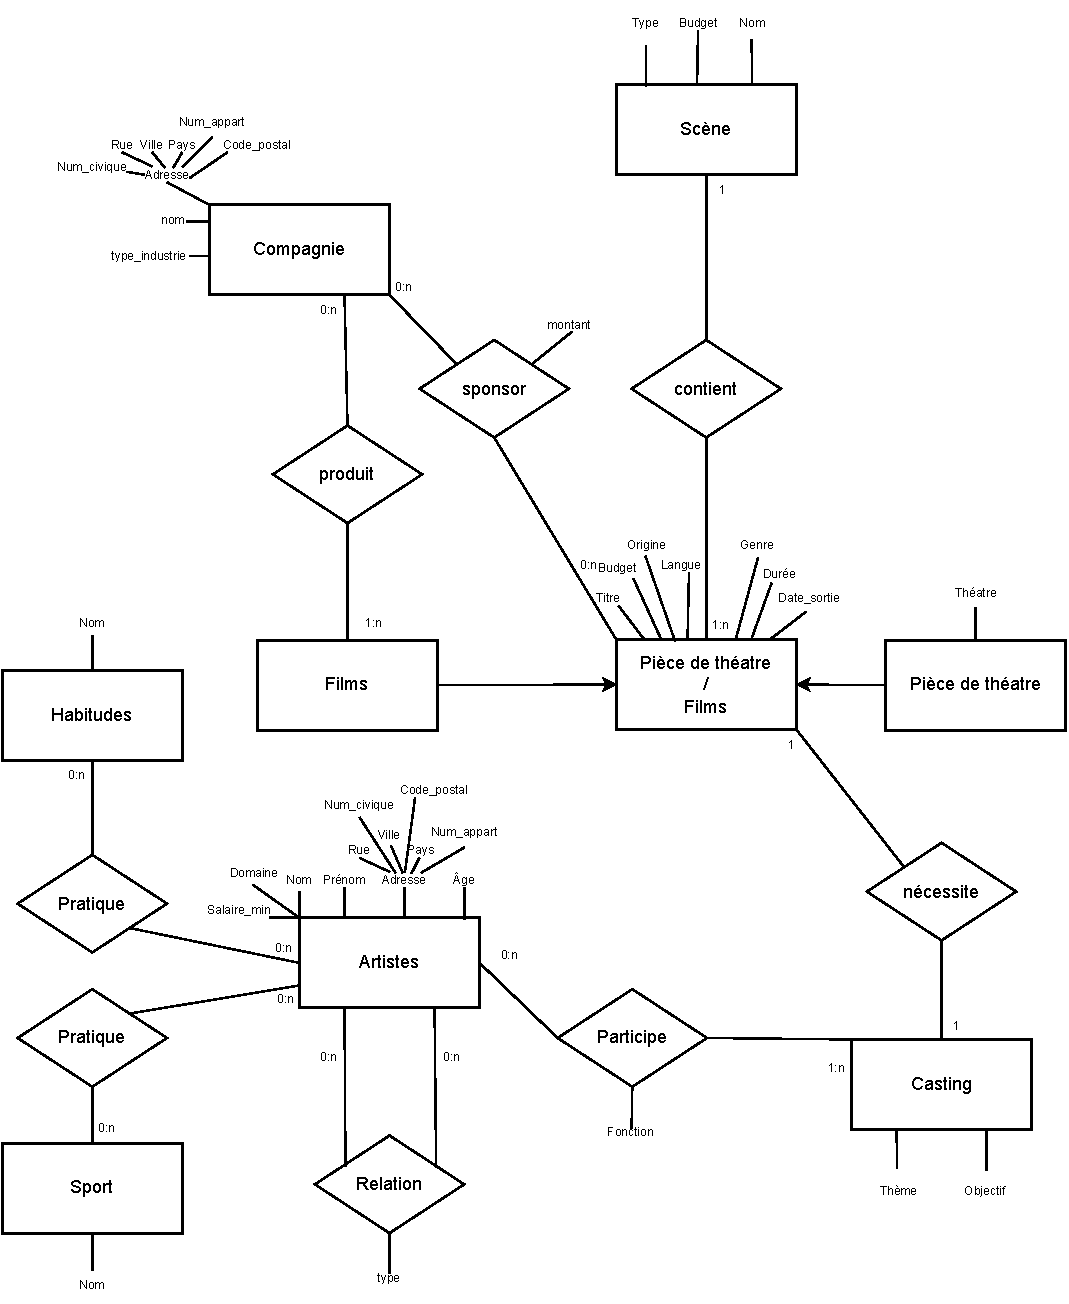
\includegraphics[scale=0.9]{modeleEA.pdf}
\end{center}


\newpage

\subsection{Modèle Relationnel}


\begin{itemize}
\item \textbf{Oeuvre}(\underline{id\_oeuvre}, titre, budget,
  date\_sortie, durée, origine, langue, genre)
  
\item \textbf{Films}(\underline{\#id\_oeuvre}, \#id\_Studio)
  
\item \textbf{Pièces\_Théâtre}(\underline{\#id\_oeuvre}, théâtre)
  
\item \textbf{Scènes}(\underline{id\_scène}, titre, budget, type,
  \#id\_oeuvre)
  
\item \textbf{Adresses}(\underline{id\_adresse},no\_civique, rue,
  ville, code\_postal, pays, no\_appartement)

\item \textbf{Habitude}(\underline{id}, nom)

\item \textbf{Sport}(\underline{id}, nom)
  
\item \textbf{Artistes}(\underline{id\_artiste}, nom, prénom,
  date\_naissance, salaire\_min, domaine, \#id\_adresse)
  
\item \textbf{Casting}(\underline{\#id\_oeuvre}, objectif, thème)

\item \textbf{Casting\_Artiste}(\underline{\#id\_artiste, \#id\_oeuvre}, fonction,
  salaire, date\_debut, date\_fin)

\item \textbf{Relation}(\underline{\#id\_artiste1, \#id\_artiste2}, type\_relation)

\item \textbf{Artiste\_Sport}(\underline{\#id\_artiste, \#id\_sport})

\item \textbf{Artiste\_Habitude}(\underline{\#id\_artiste, \#id\_habitude})

\item \textbf{Compagnies}(\underline{id\_compagnie}, nom,
  type\_industrie, \#id\_adresse)
  
\item \textbf{Sponsors}(\underline{\#id\_oeuvres \#id\_compagnie},
  montant)
  
\item \textbf{Producteurs}(\underline{\#id\_oeuvres
    \#id\_compagnie})

\end{itemize}

\newpage
\subsection{Dépendances fonctionnelles}


\textbf{Oeuvre}(\underline{id\_oeuvre}, titre, budget, date\_sortie,
durée, origine, langue, genre)

\begin{itemize}
\item id\_oeuvre $\rightarrow$ titre, budget, date\_sortie, durée,
  origine, langue, genre
\end{itemize}

\vspace{2mm}
\noindent
\textbf{Addresses}(\underline{id\_adresse}, no\_civique, rue, ville, code\_postal, pays, no\_appartement)

\begin{itemize}
\item id\_adresse $\rightarrow$ no\_civique, rue, ville, code\_postal, pays, no\_appartement
\end{itemize}

\vspace{2mm}
\noindent
\textbf{Habitude}(\underline{id\_habitude}, nom)

\begin{itemize}
\item id\_habitude $\rightarrow$ nom
\item nom $\rightarrow$ id\_habitude
\end{itemize}

\vspace{2mm}
\noindent
\textbf{Sport}(\underline{id\_sport}, nom)

\begin{itemize}
\item id\_sport $\rightarrow$ nom
\item nom $\rightarrow$ id\_sport
\end{itemize}

\vspace{2mm}
\noindent
\textbf{Compagnies}(\underline{id\_compagnie}, nom, type\_industrie, \#id\_adresse)

\begin{itemize}
\item id\_compagnie $\rightarrow$ nom, type\_industrie, id\_adresse
\end{itemize}

\vspace{2mm}
\noindent
\textbf{Films}(\#\underline{id\_oeuvre}, \#\underline{id\_studio})

\begin{itemize}
\item id\_oeuvre $\rightarrow$ id\_studio
\end{itemize}

\vspace{2mm}
\noindent
\textbf{Pièce\_Théâtre}(\#\underline{id\_oeuvre}, théâtre)

\begin{itemize}
\item id\_oeuvre $\rightarrow$ théâtre
\end{itemize}

\vspace{2mm}
\noindent
\textbf{Scènes}(\underline{id\_scène}, titre, budget, type, \#id\_oeuvre)

\begin{itemize}
\item id\_scène $\rightarrow$ titre, budget, type, id\_oeuvre
\item id\_oeuvre, titre $\rightarrow$ id\_scène, type, budget
\end{itemize}

\vspace{2mm}
\noindent
\textbf{Artiste}(\underline{id\_artiste}, nom, prénom, date\_naissance, salaire\_min, domaine, \#id\_adresse)

\begin{itemize}
\item id\_artiste $\rightarrow$ nom, prénom, date\_naissance, salaire\_min, domaine, id\_adresse
\end{itemize}

\vspace{2mm}
\noindent
\textbf{Casting}(\#\underline{id\_oeuvre}, objectif, thème)

\begin{itemize}
\item id\_oeuvre $\rightarrow$ objectif, thème
\end{itemize}

\vspace{2mm}
\noindent
\textbf{Sponsor}(\#\underline{id\_oeuvre}, \#\underline{id\_compagnie}, montant)

\begin{itemize}
\item id\_oeuvre, id\_compagnie $\rightarrow$ montant
\end{itemize}

\vspace{2mm}
\noindent
\textbf{Producteur}(\#\underline{id\_oeuvre}, \#\underline{id\_compagnie})

\newpage
\noindent
\textbf{Casting\_Artiste}(\#\underline{id\_artiste}, \#\underline{id\_oeuvre}, fonction, salaire, date\_début, date\_fin)

\begin{itemize}
\item id\_artiste, id\_oeuvre $\rightarrow$ fonction, salaire, date\_début, date\_fin
\end{itemize}

\vspace{2mm}
\noindent
\textbf{Relation}(\#\underline{id\_artiste1}, \#\underline{id\_artiste2}, type\_relation)

\begin{itemize}
\item id\_artiste1, id\_artiste2 $\rightarrow$ type\_relation
\end{itemize}

\vspace{2mm}
\noindent
\textbf{Artiste\_Sport}(\#\underline{id\_artiste}, \#\underline{id\_sport})

\vspace{2mm}
\noindent
\textbf{Artiste\_Habitude}(\#\underline{id\_artiste}, \#\underline{id\_habitude})



\subsection{Normalisation}
Ici il est important de noter que nous avons modélisé les relations
en prenant en compte que nous avions à normaliser la base de données
par la suite. Nous avons donc pris soin de décomposer les relations
au maximum.
\subsubsection*{Transformation en 1NF}
Ici rien à faire, car les tables sont déjà en 1NF: chaque attribut est
atomique.

\subsubsection*{Transformation en 2NF}
Ici rien à faire, car les tables sont déjà en 2NF: chaque attribut
non-clé ne dépend pas d'une partie de la clé.

\subsubsection*{Transformation en 3NF}
Ici rien à faire, car les tables sont déjà en 3NF:
tout attribut n'appartenant pas à la clé ne dépend pas d'un attribut non clé
\vspace{5mm}
\section{SQL}

Tout les fichiers sql sont dans le dossier
\href{https://github.com/ZGaillard/projet_session_2935/tree/main/database}{\color{blue}{\underline{database}}}.
\subsection{LDD}
Le fichier
\href{https://github.com/ZGaillard/projet_session_2935/blob/main/database/CreateUpdated.sql}{\color{blue}{\underline{CreateUpdated.sql}}}
contient la création de la base de données et des tables.

\subsection{LMD}
Le fichier
\href{https://github.com/ZGaillard/projet_session_2935/blob/main/database/Populate.sql}{\color{blue}{\underline{populate.sql}}}
contient le peuplement de la base de données. Ce fichier utilise des
procédures stockées pour generer certaines données aléatoires.
Les procédures stockées sont définies dans les fichiers 
  \href{https://github.com/ZGaillard/projet_session_2935/blob/main/database/GenCastingArtistes.sql}{\color{blue}{\underline{GenCastingArtistes.sql}}},
  \href{https://github.com/ZGaillard/projet_session_2935/blob/main/database/GenArtisteSport.sql}{\color{blue}{\underline{GenArtisteSport.sql}}}
  et
  \href{https://github.com/ZGaillard/projet_session_2935/blob/main/database/GenArtisteHabit.sql
  }{\color{blue}{\underline{GenArtisteHabit.sql}}}

  \newpage
\subsection{Requêtes}
Nous avons d'abord créer dix requêtes pour tester la base de
donnée. Ces requêtes sont dans le fichier
\href{https://github.com/ZGaillard/projet_session_2935/blob/main/database/request.sql}{\color{blue}{\underline{request.sql}}}.\n
Par la suite, nous avons créé une classe python pour exécuter des
requêtes SQL. Cette classe est dans le fichier \href{
  https://github.com/ZGaillard/projet_session_2935/blob/main/app/DBManager.py}{\color{blue}{\underline{DBManager.py}}}.
Cette classe utilise \texttt{pymssql} pour se connecter à la base de
données. Elle permet d'exécuter des requêtes simples et de récupérer
les résultats. Elle permet aussi d'exécuter des procédures stockées.\n
Durant le développement de l'application, nous avons trouvé qu'il
était plus judicieux de créer des procédures stockées pour les
requêtes qui nécessitaient des requêtes plus complexes. Ces procédures
stockées sont dans les fichiers :

\begin{itemize}
\item
  \href{https://github.com/ZGaillard/projet_session_2935/blob/main/database/DefAddAdresse.sql}{\color{blue}{\underline{DefAddAdresse.sql}}}

\item
  \href{https://github.com/ZGaillard/projet_session_2935/blob/main/database/DefAddArtist.sql}{\color{blue}{\underline{DefAddArtist.sql}}}

\item
  \href{https://github.com/ZGaillard/projet_session_2935/blob/main/database/DefAddCasting.sql}{\color{blue}{\underline{DefAddCasting.sql}}}

\item
  \href{https://github.com/ZGaillard/projet_session_2935/blob/main/database/DefAddMovies.sql}{\color{blue}{\underline{DefAddMovies.sql}}}

\item
  \href{https://github.com/ZGaillard/projet_session_2935/blob/main/database/DefAddPlays.sql}{\color{blue}{\underline{DefAddPlays.sql}}}

\item
  \href{https://github.com/ZGaillard/projet_session_2935/blob/main/database/DefGetArtistHabit.sql}{\color{blue}{\underline{DefGetArtistHabit.sql}}}
  
\item
  \href{https://github.com/ZGaillard/projet_session_2935/blob/main/database/DefGetArtistRelations.sql}{\color{blue}{\underline{DefGetArtistRelations.sql}}}
  
\item
  \href{https://github.com/ZGaillard/projet_session_2935/blob/main/database/DefGetArtistSports.sql}{\color{blue}{\underline{DefGetArtistSports.sql}}}
  
\item
  \href{https://github.com/ZGaillard/projet_session_2935/blob/main/database/DefGetArtists.sql}{\color{blue}{\underline{DefGetArtists.sql}}}
  
\item
  \href{https://github.com/ZGaillard/projet_session_2935/blob/main/database/DefGetCastingArtists.sql}{\color{blue}{\underline{DefGetCastingArtists.sql}}}
  
\item
  \href{https://github.com/ZGaillard/projet_session_2935/blob/main/database/DefGetCastings.sql}{\color{blue}{\underline{DefGetCastings.sql}}}
  
\item
  \href{https://github.com/ZGaillard/projet_session_2935/blob/main/database/DefGetCompagnies.sql}{\color{blue}{\underline{DefGetCompagnies.sql}}}
  
\item
  \href{https://github.com/ZGaillard/projet_session_2935/blob/main/database/DefGetMovies.sql}{\color{blue}{\underline{DefGetMovies.sql}}}

\item
  \href{https://github.com/ZGaillard/projet_session_2935/blob/main/database/DefGetPlays.sql}{\color{blue}{\underline{DefGetPlays.sql}}}

\end{itemize}


\newpage
\section{Application}
Nous avons choisi de développer l'application en python. Nous avons
utilisé la librairie \texttt{tkinter} ainsi que \texttt{ttkbootstrap}
pour un design plus moderne des widgets.\n
La base de données est en SQL Server. Nous avons utilisé la librairie
\texttt{pymssql} pour se connecter à la base de données.\n\n
L'application permet de visualiser les artistes, leur relations
leurs habitudes et sports. Elle permet aussi de visualiser les
castings et les artistes qui y participent, ainsi que les films et les
pièces de théâtre présents dans la base de données.\n
Une fonctionnalité de recherche est aussi disponible lorsqu'on
visualise les données.\n
Nous avons aussi ajouté une fonctionnalité pour ajouter des données
dans la base de données directement depuis l'application.\n
Voici quelques captures d'écran de l'application:

\vspace{10mm}

\subsection{Page d'accueil}

\begin{center}
  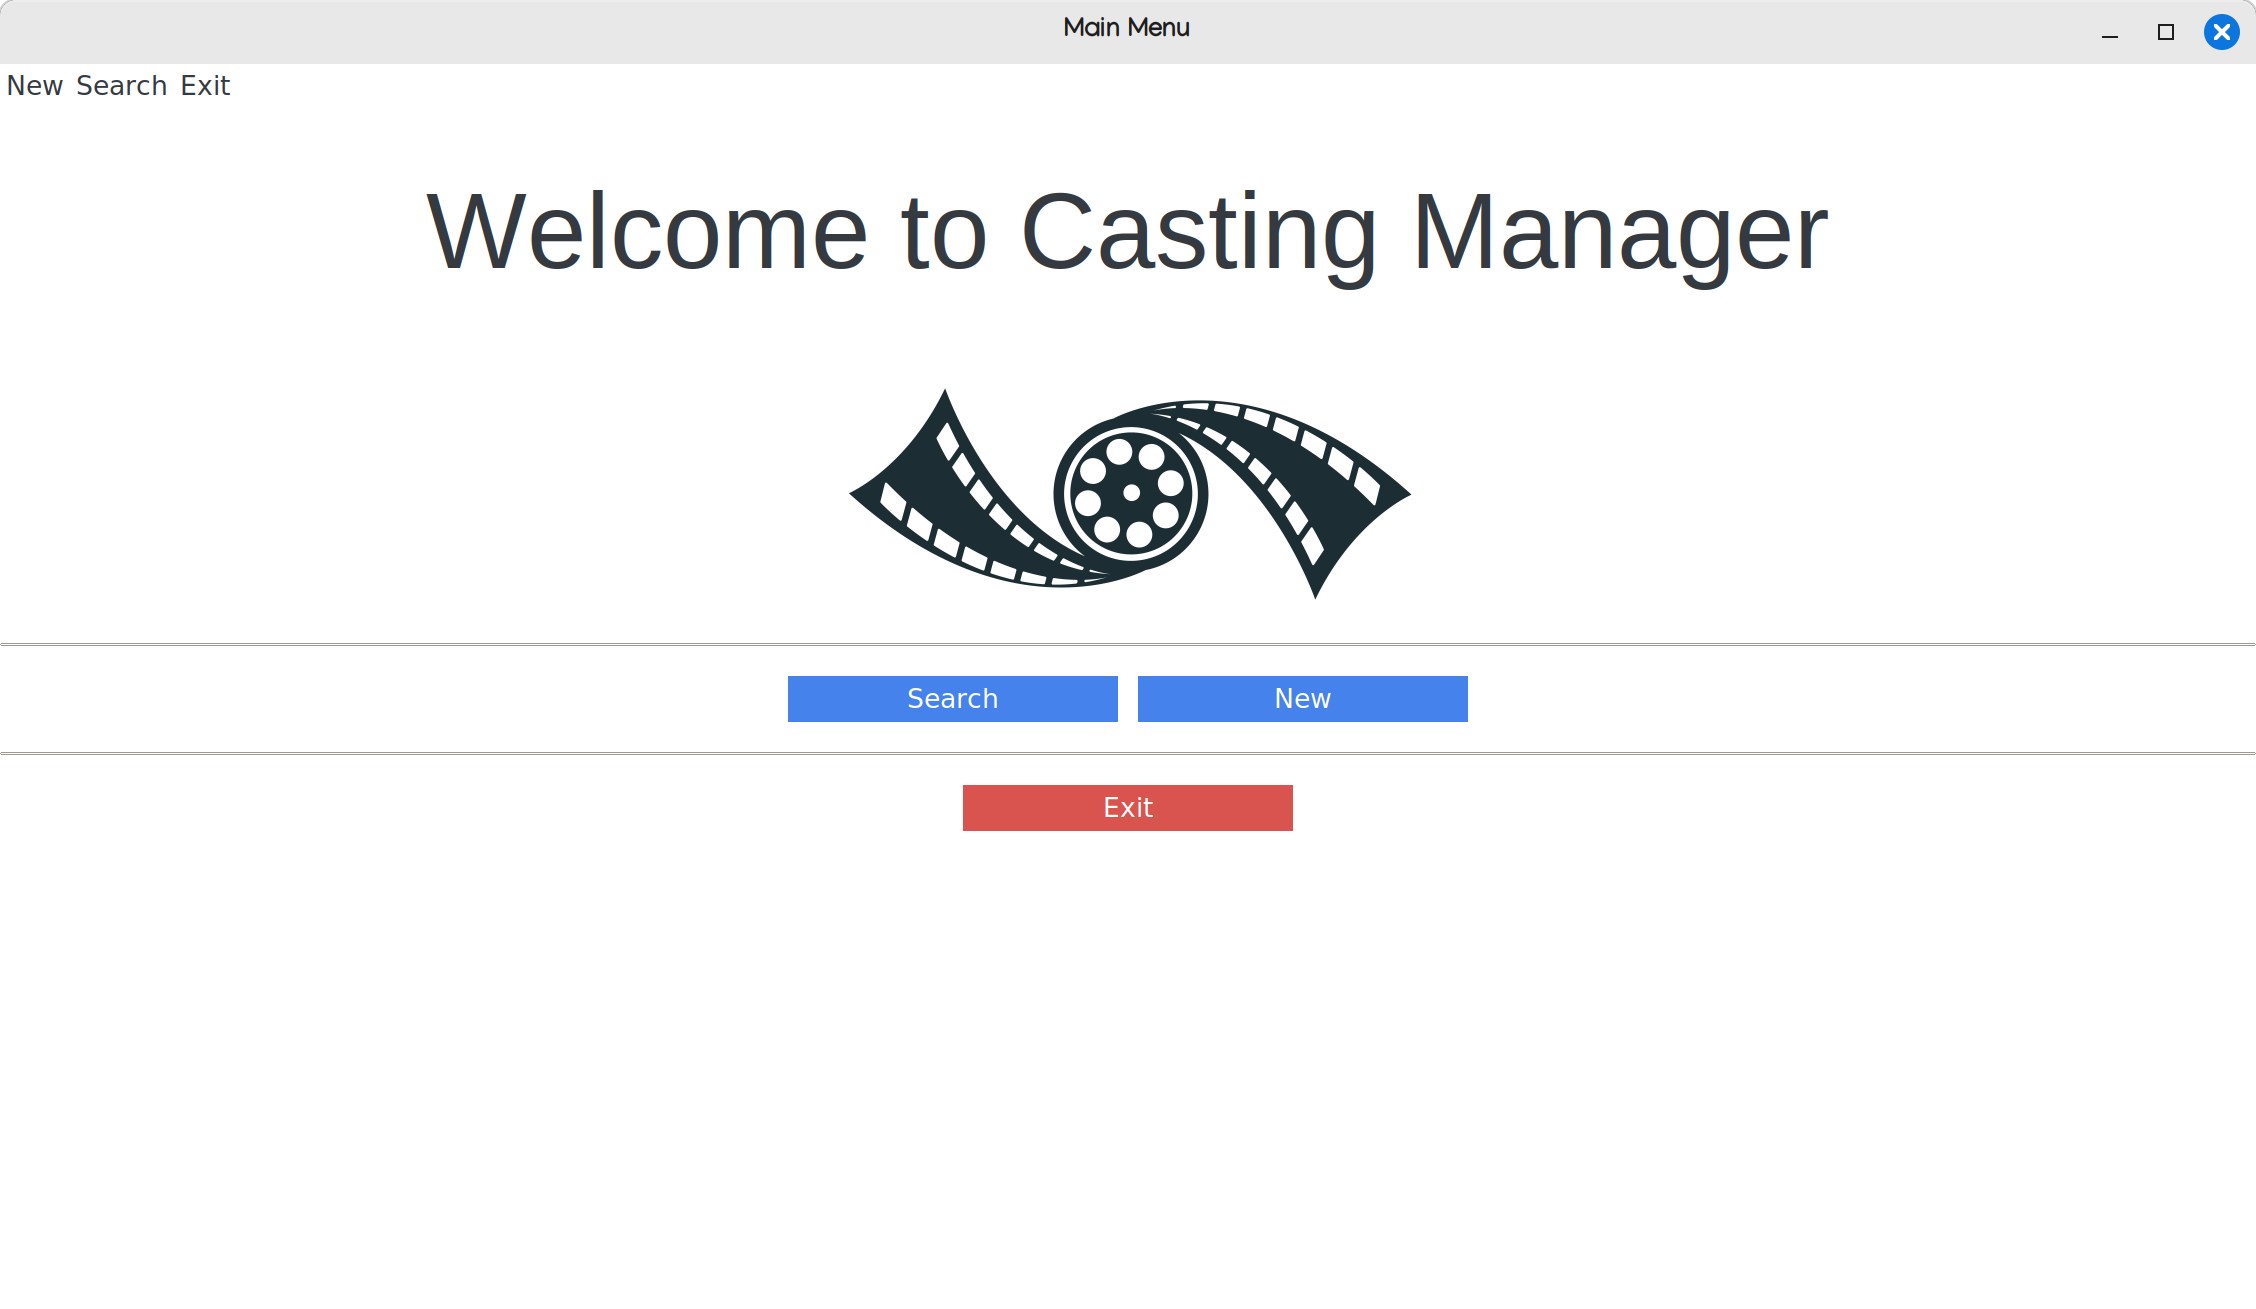
\includegraphics[scale=0.16]{home.png}
\end{center}

\newpage
\subsection{Menu de navigation}
Nous avons choisi d'ajouté un ``menubar'' pour naviguer entre les
différentes pages de l'application à partir de n'importe quelle page.
\begin{center}
  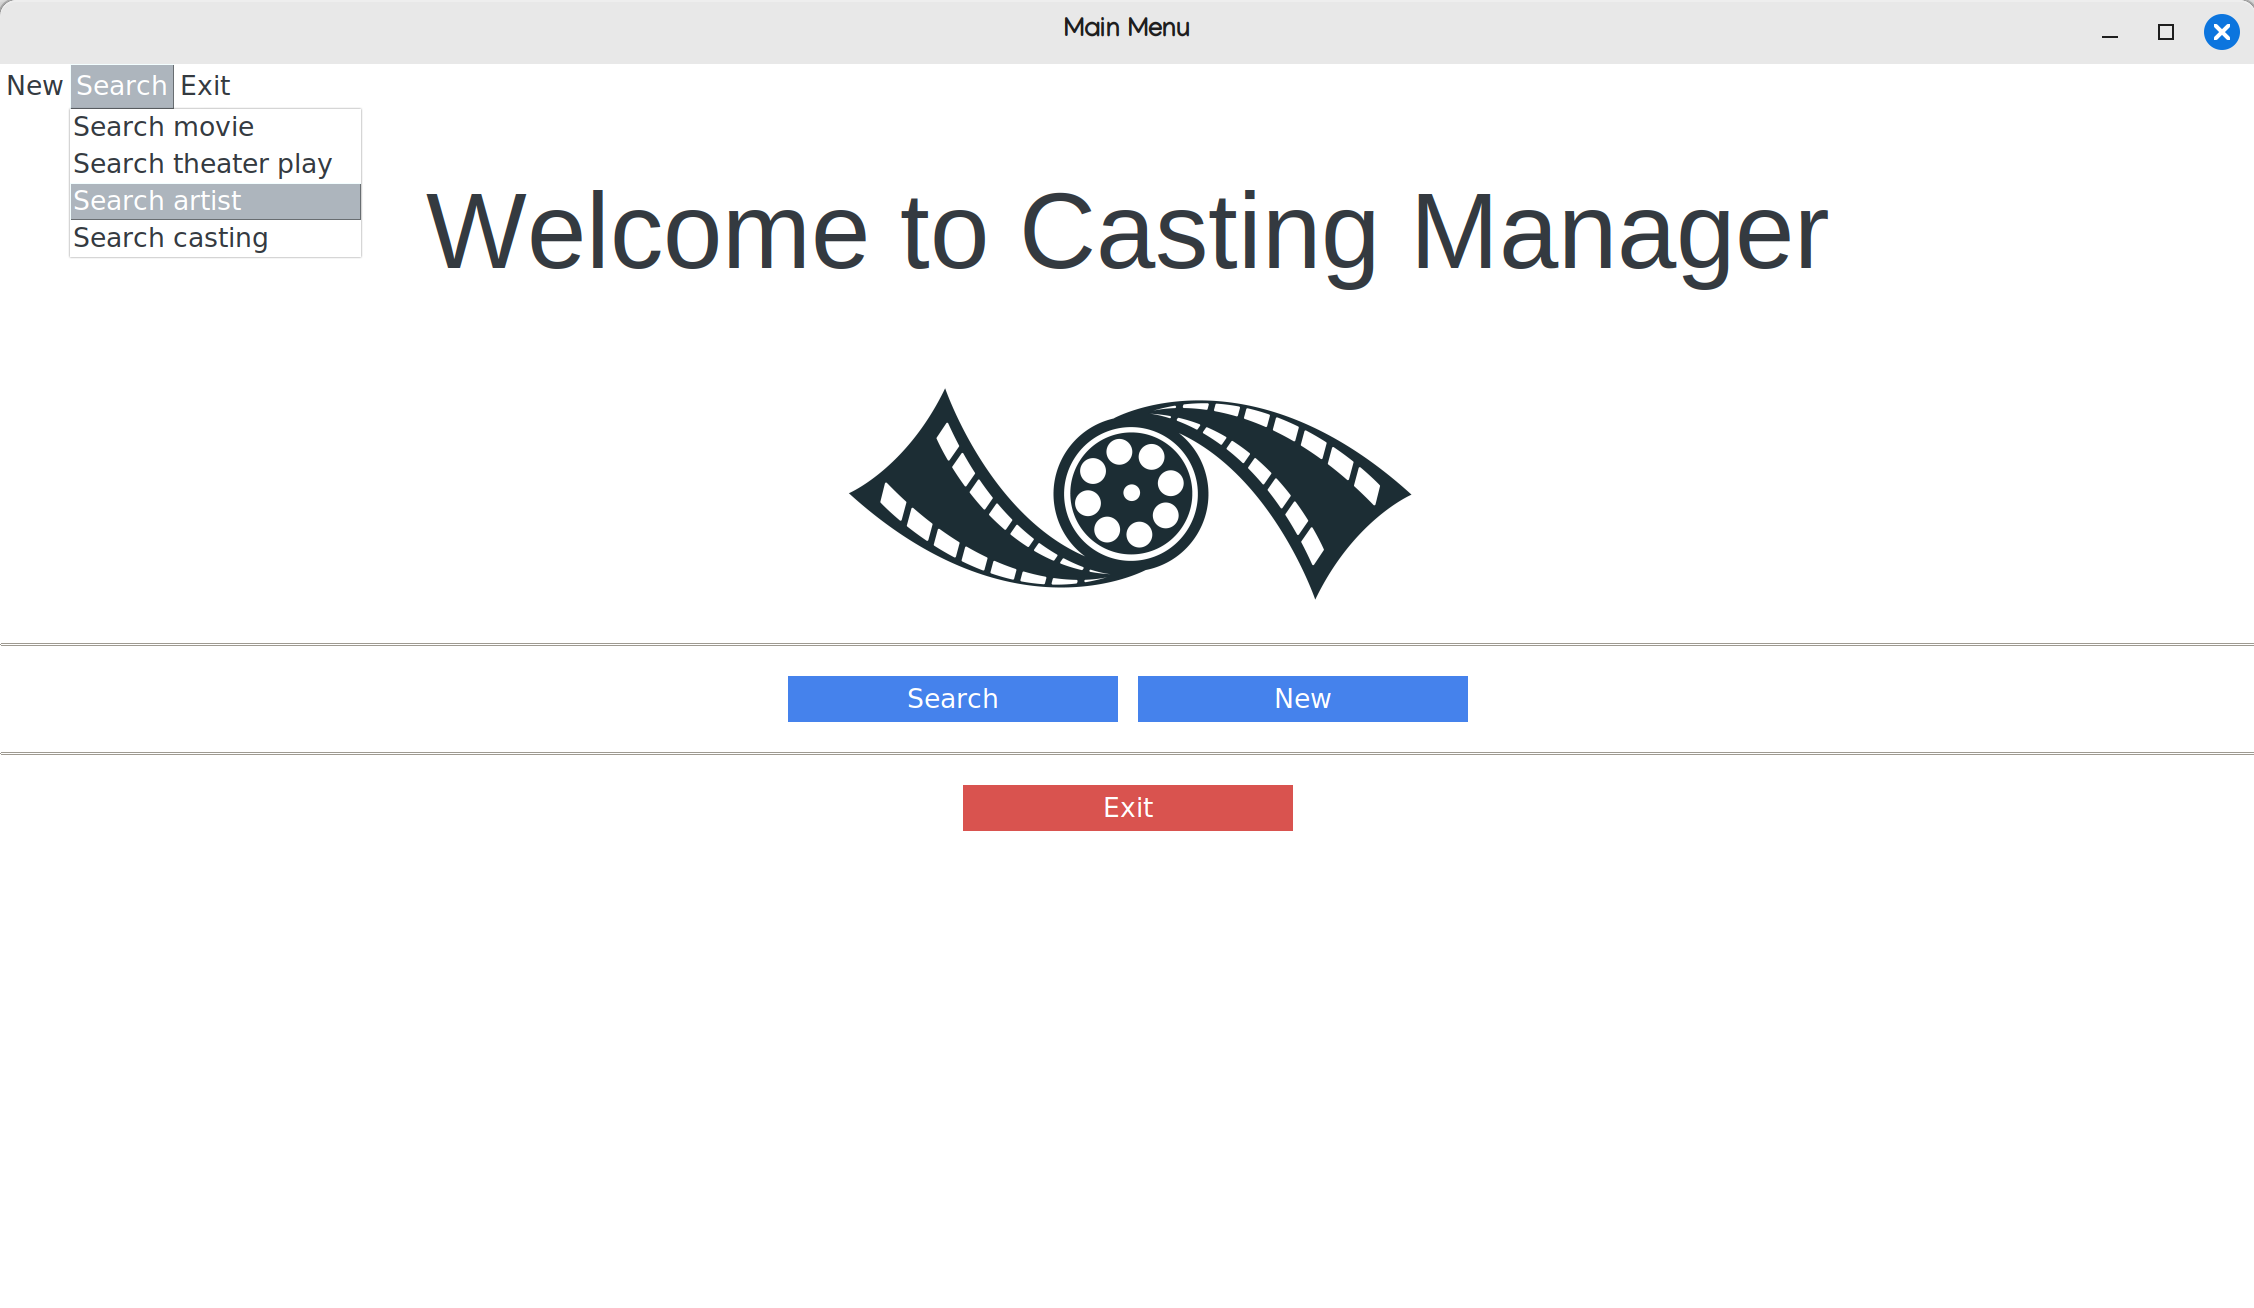
\includegraphics[scale=0.16]{menubar.png}
  
\end{center}


\subsection{Menu de recherche}

\begin{center}
  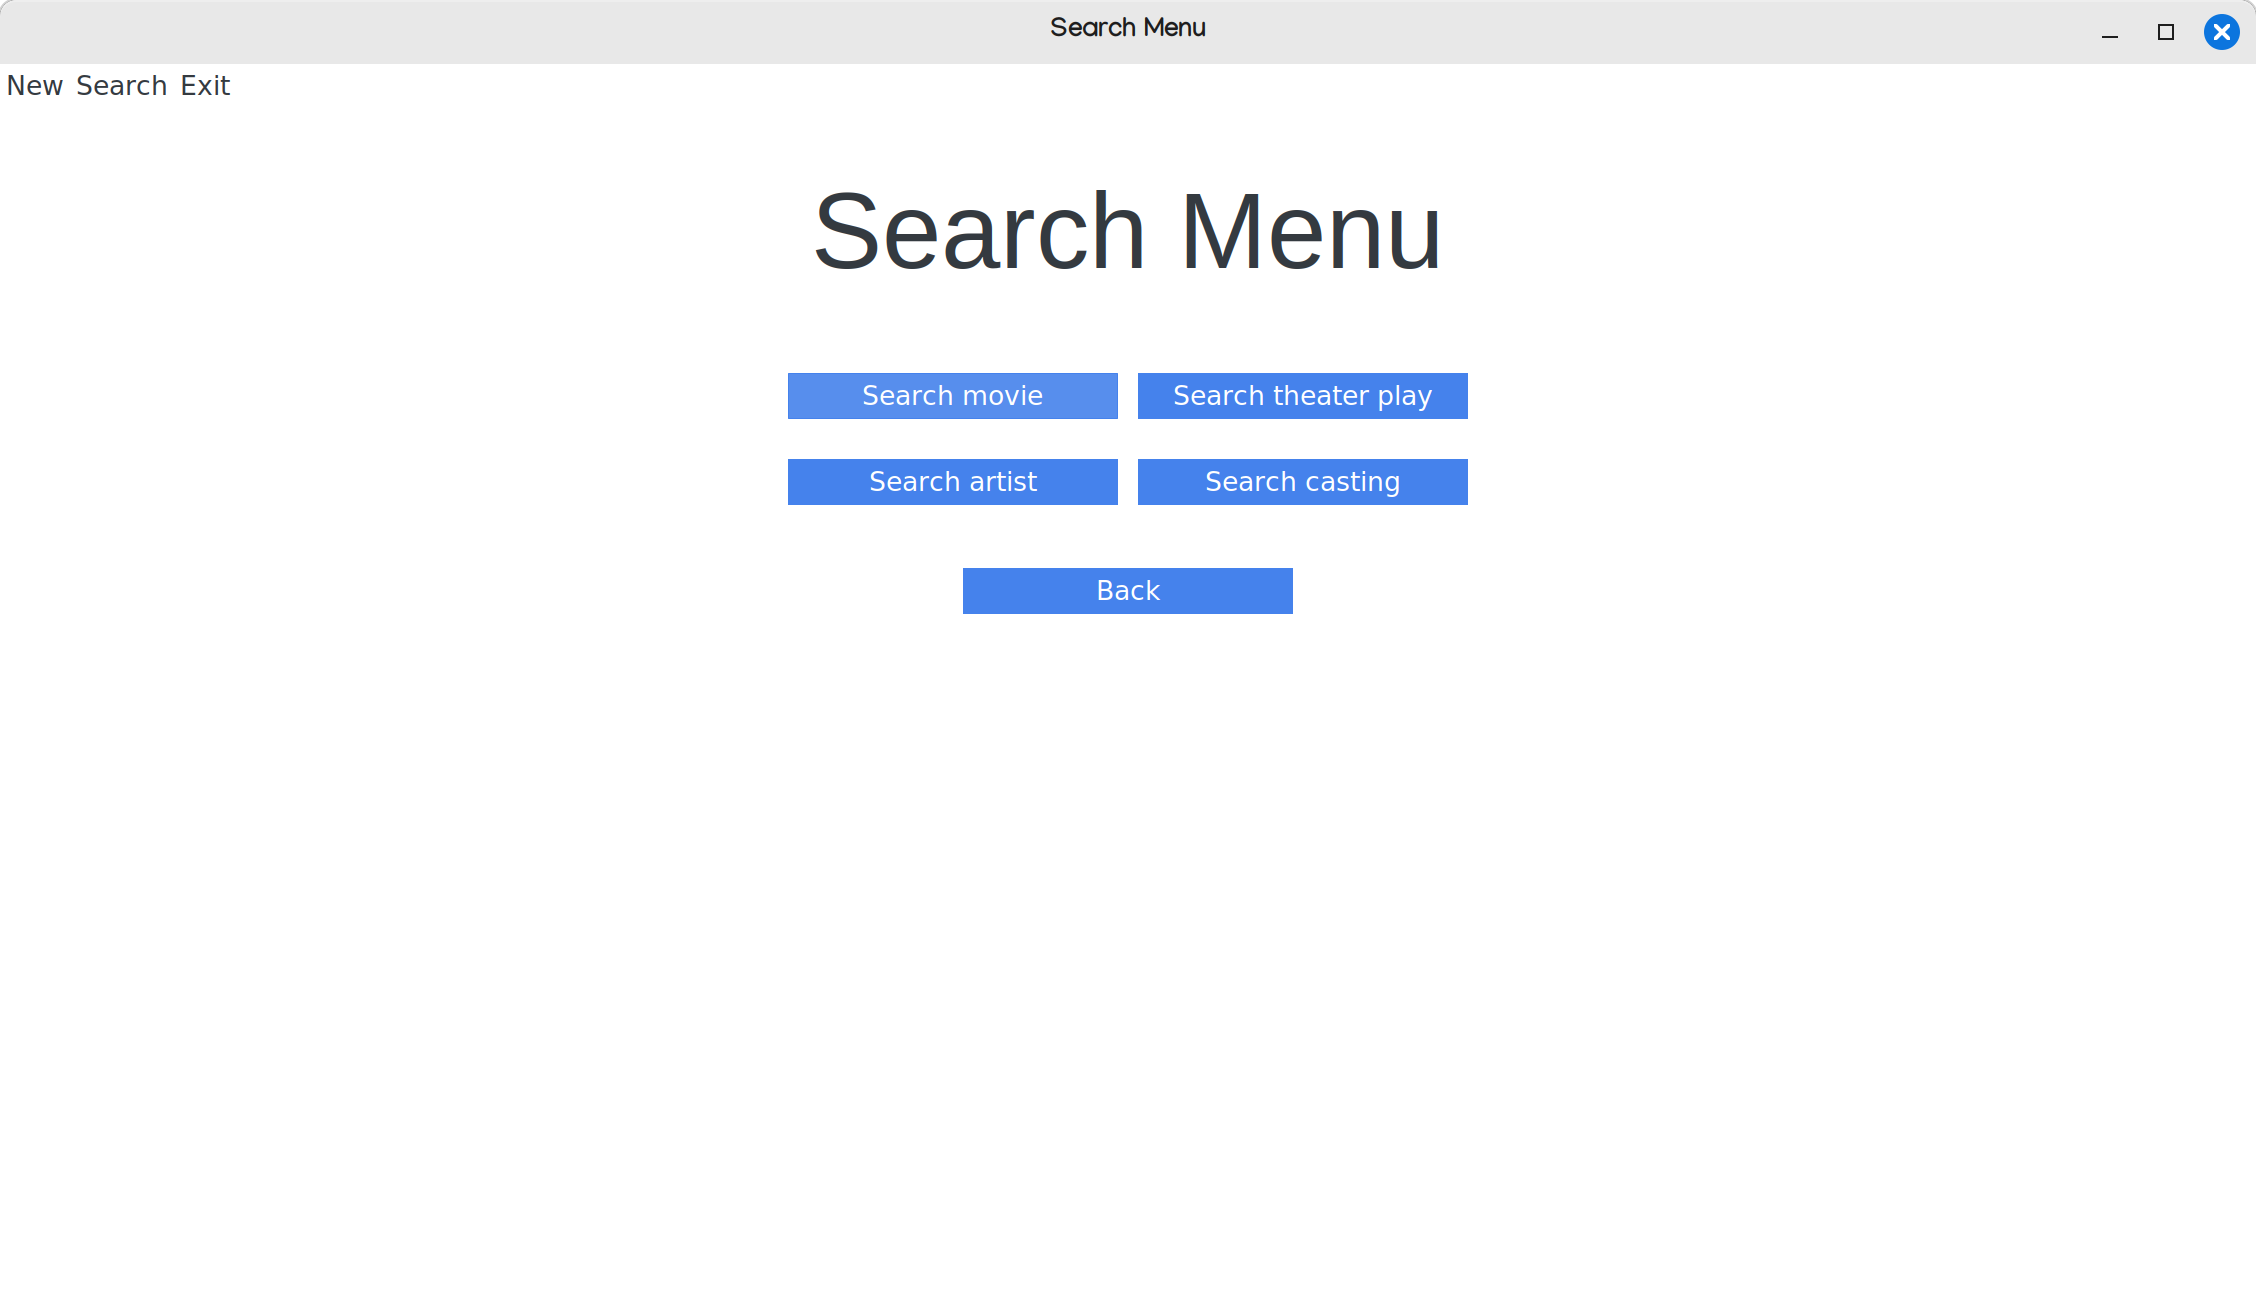
\includegraphics[scale=0.16]{search.png}
\end{center}

\subsection{Page de visualisation des artistes}

\begin{center}
  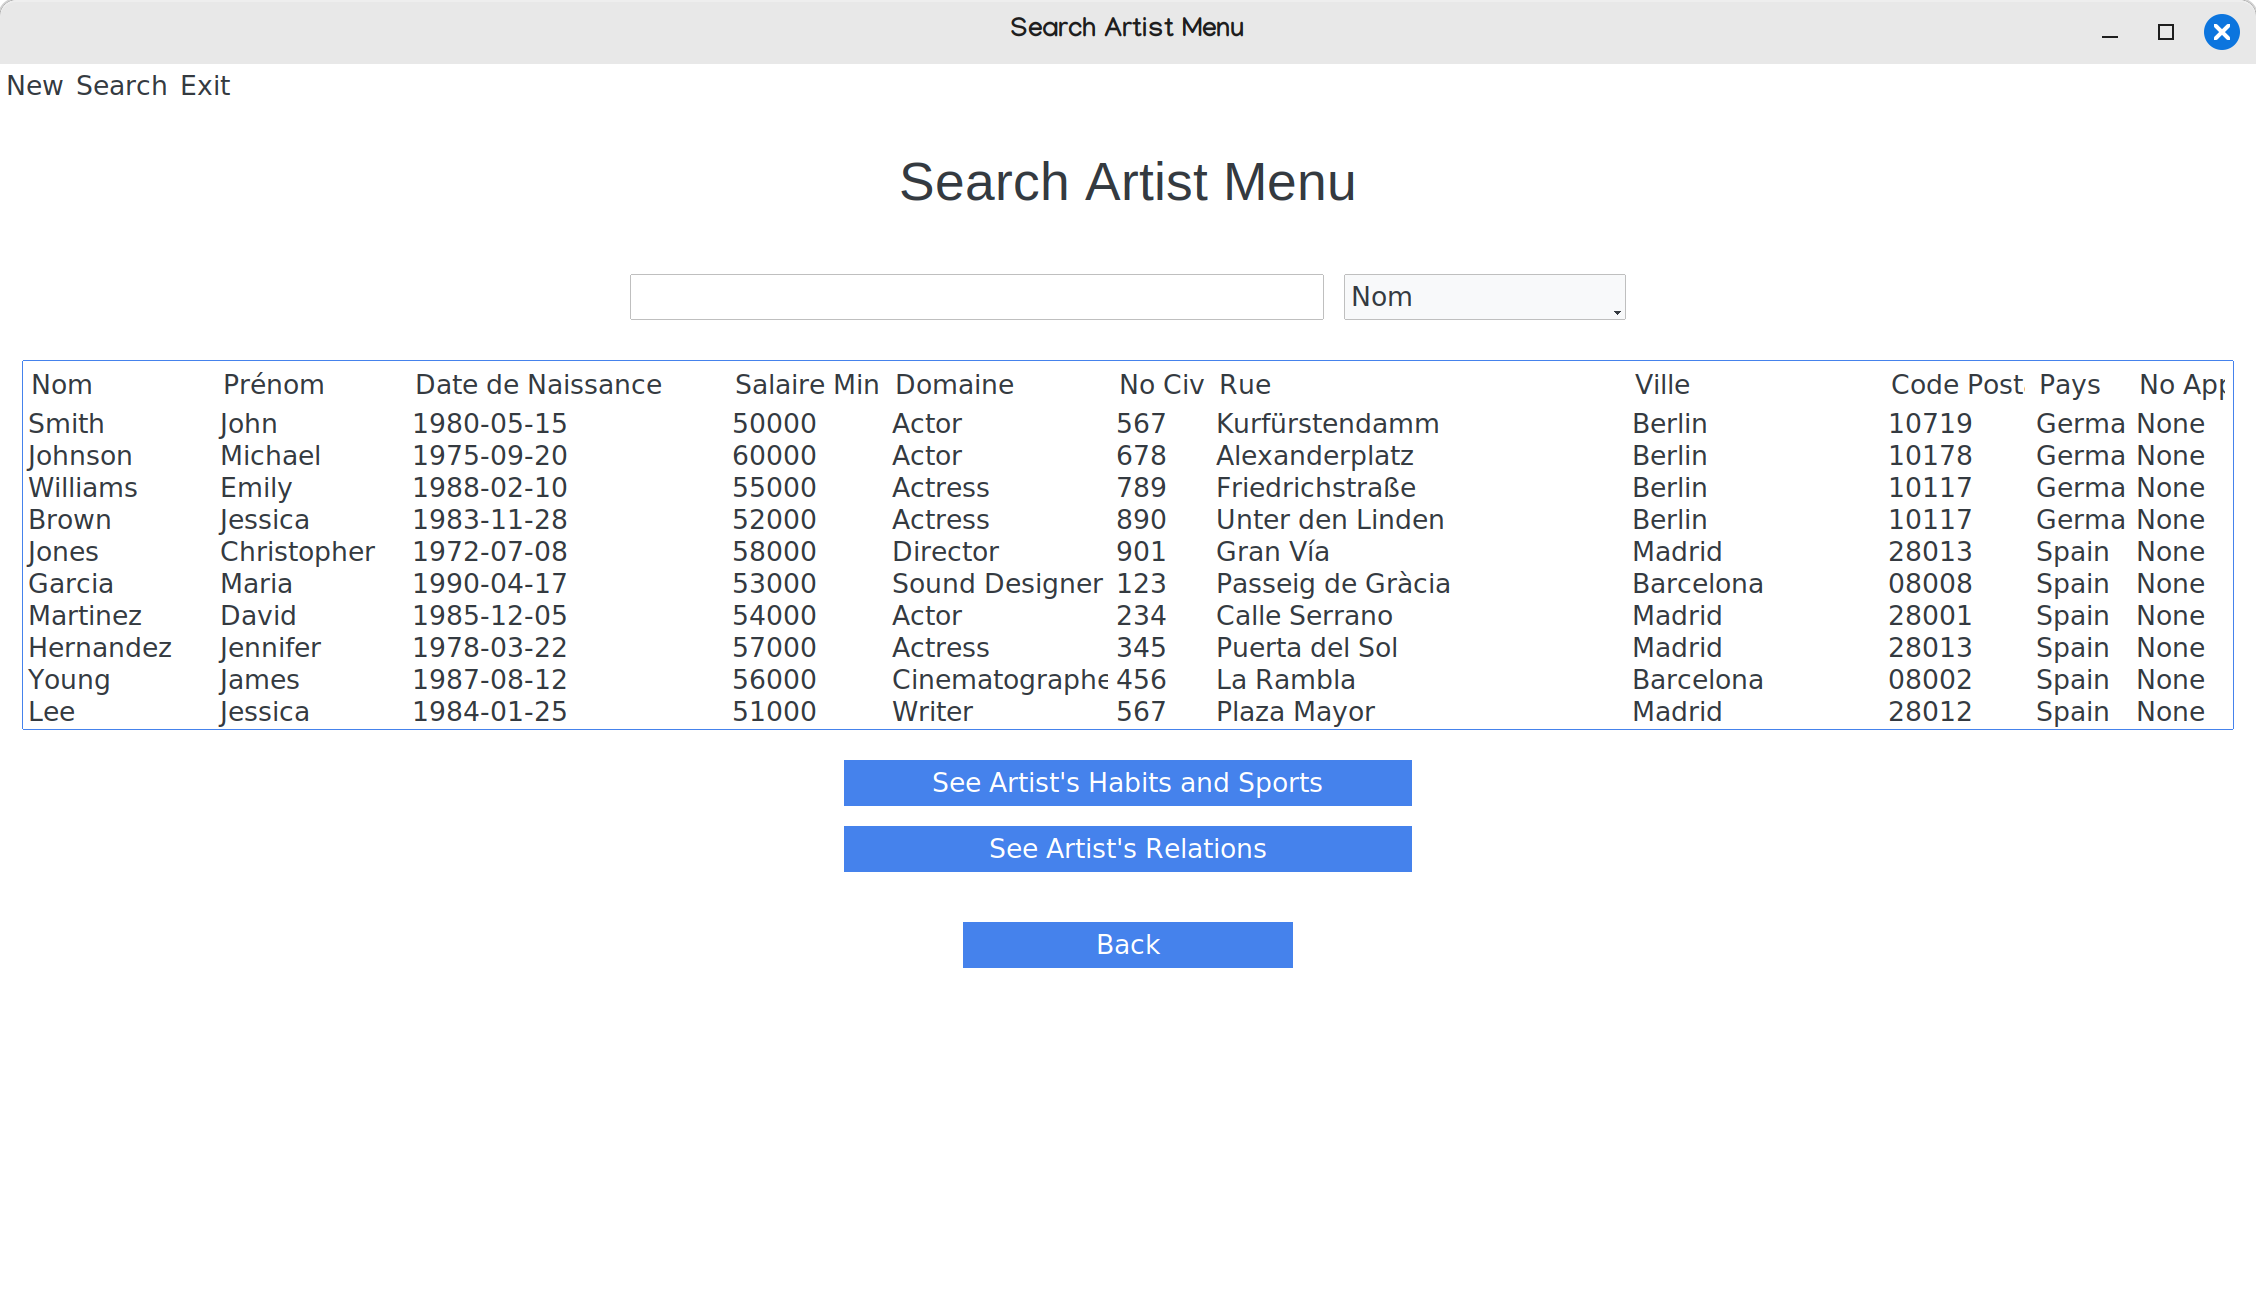
\includegraphics[scale=0.16]{searchartist.png}\n
  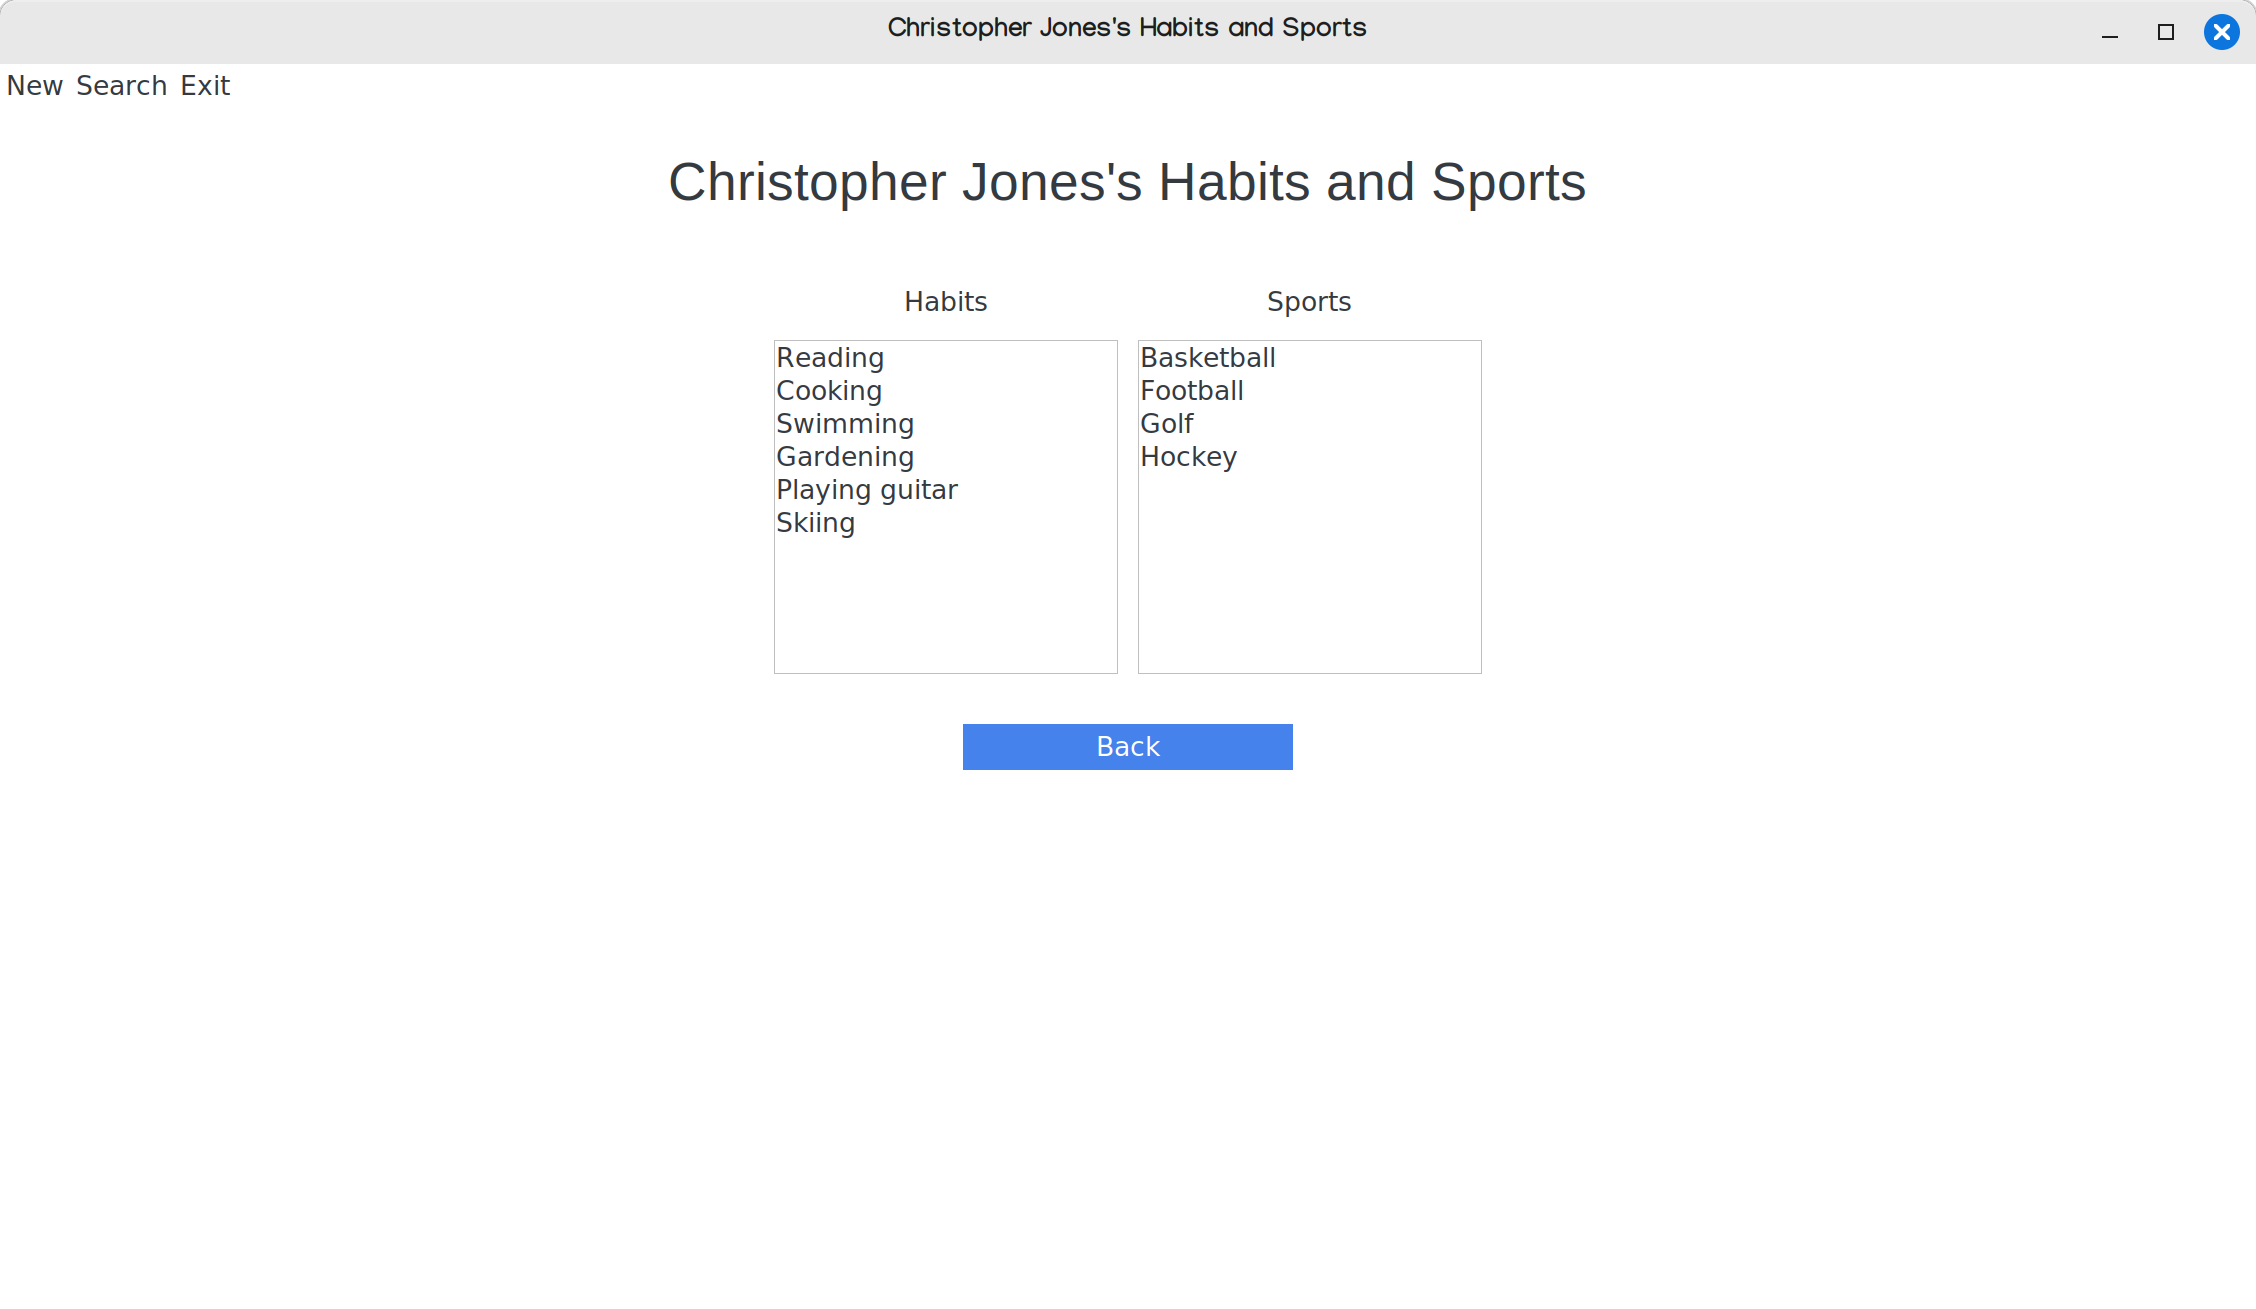
\includegraphics[scale=0.16]{habitsports.png}\n
  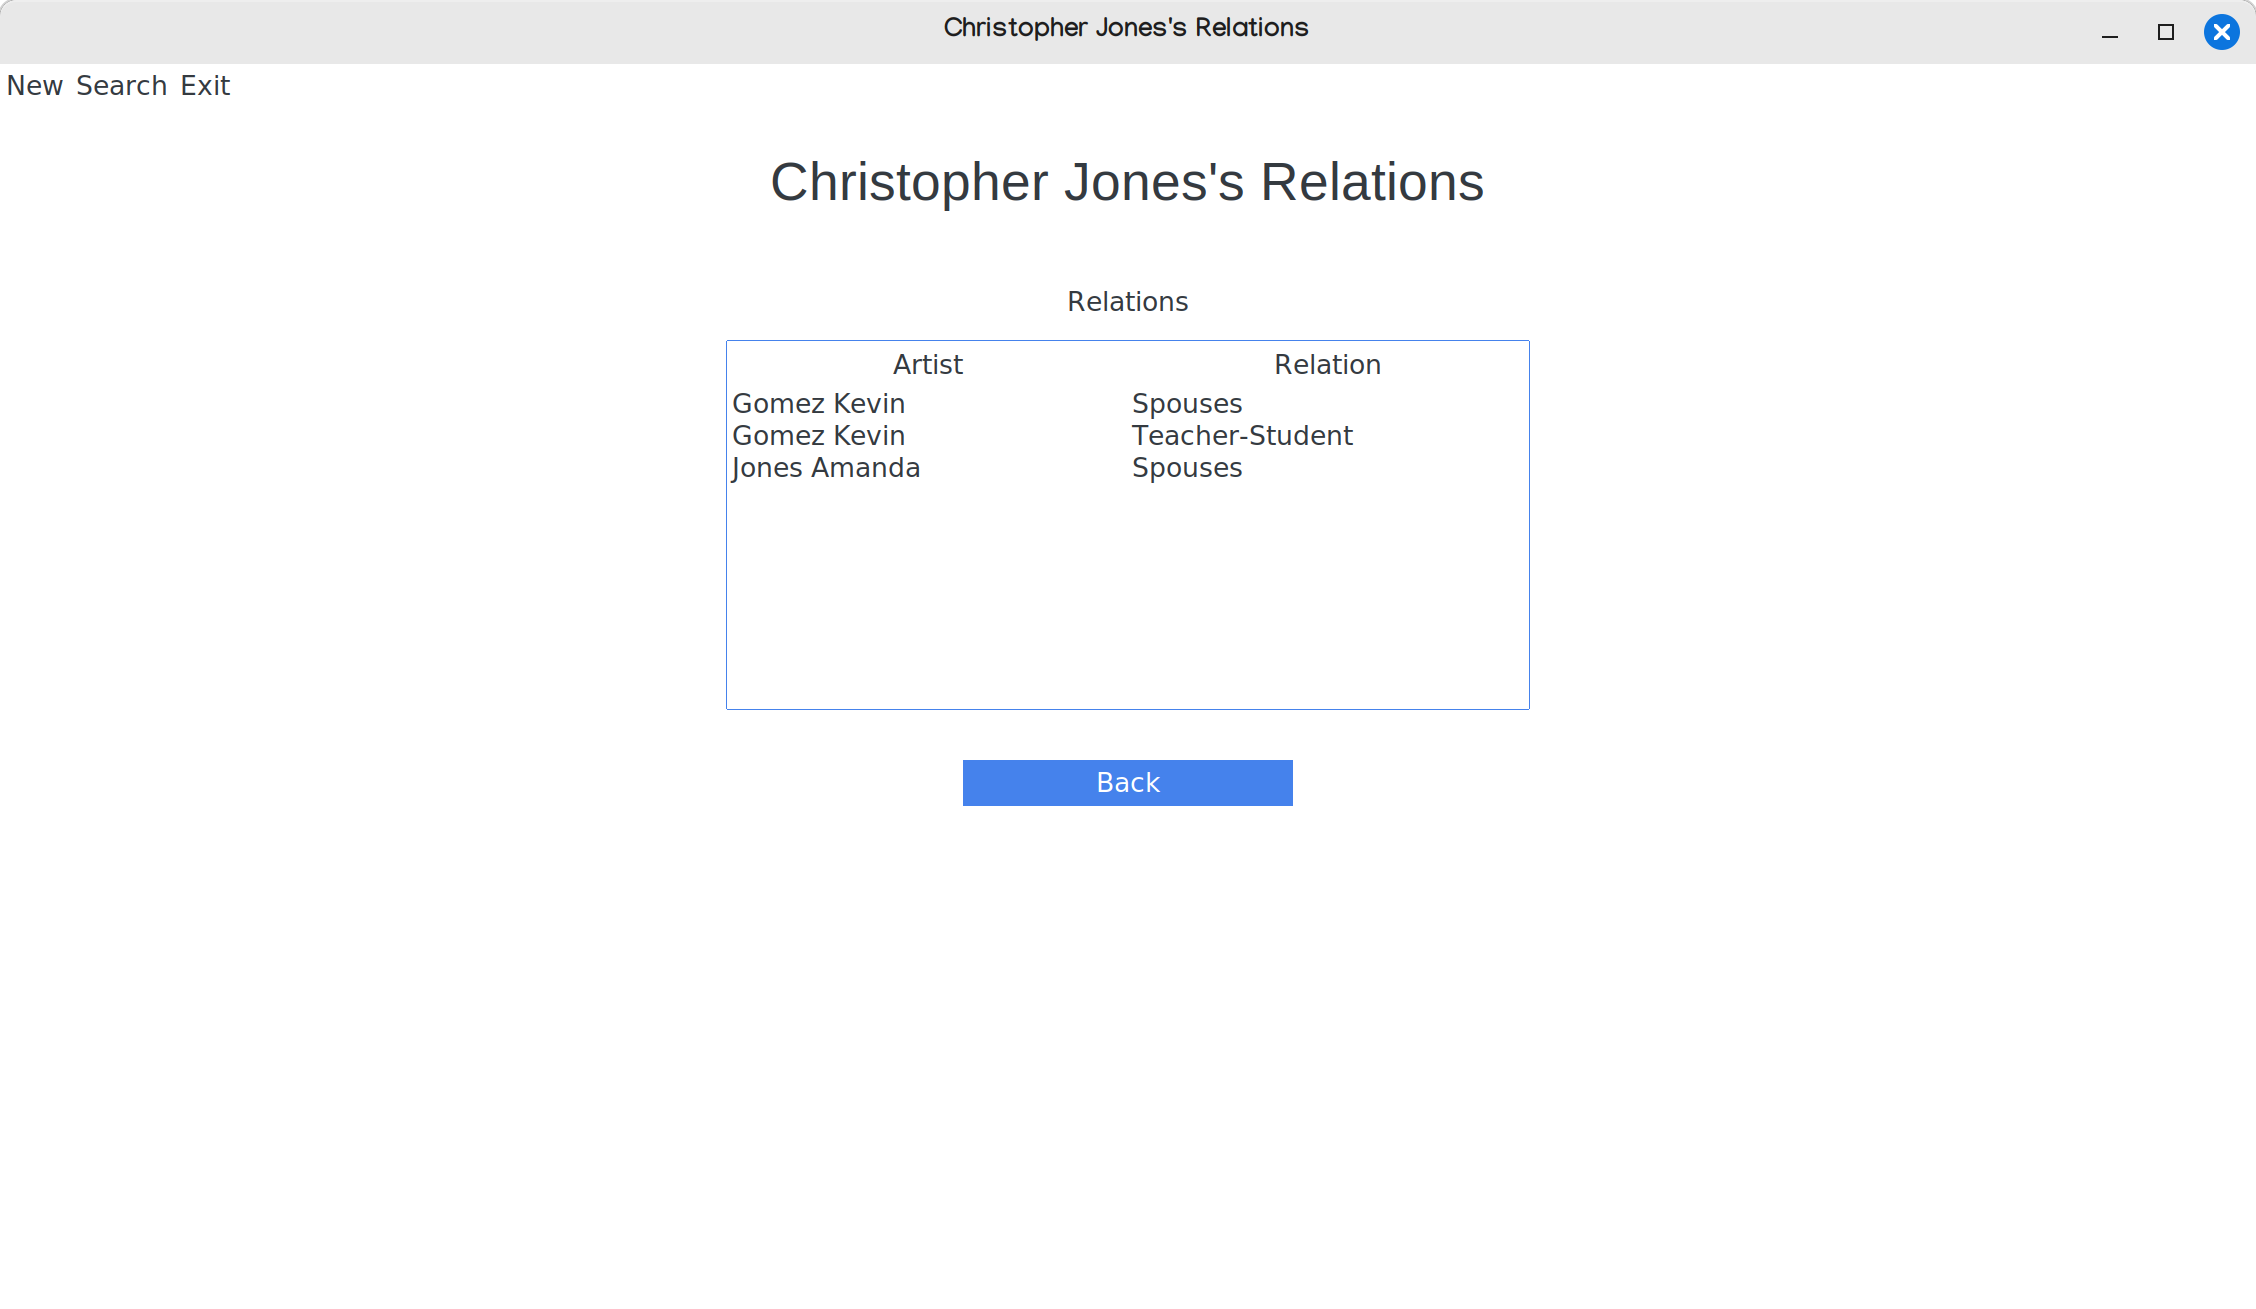
\includegraphics[scale=0.16]{artistrelation.png}
\end{center}

\subsection{Page de visualisation des castings}
\begin{center}
  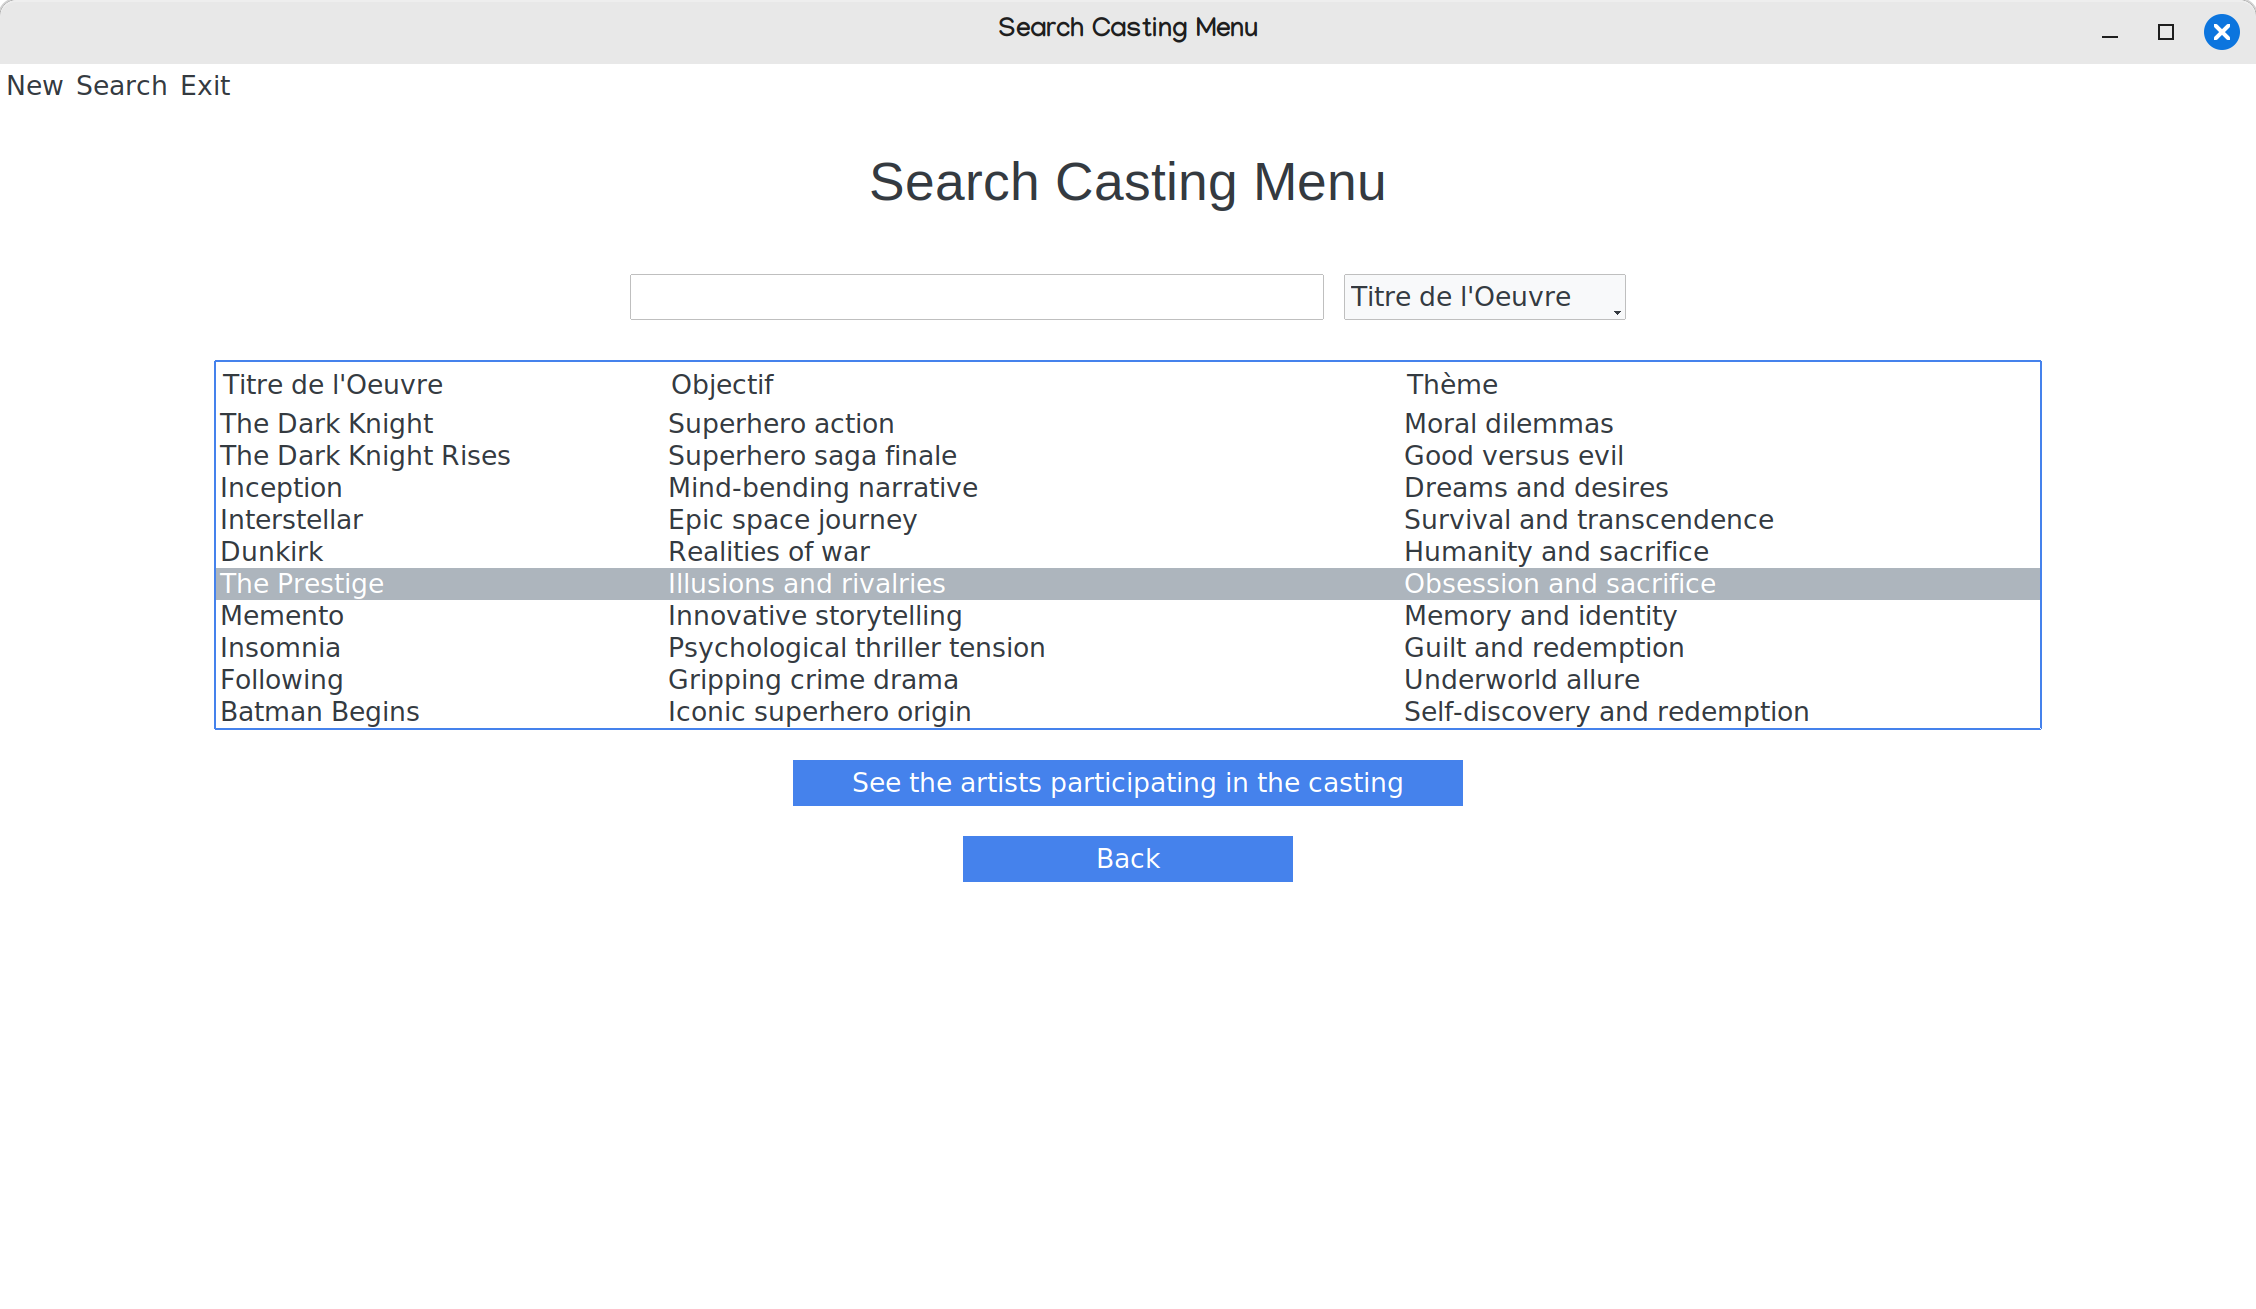
\includegraphics[scale=0.16]{casting.png}
  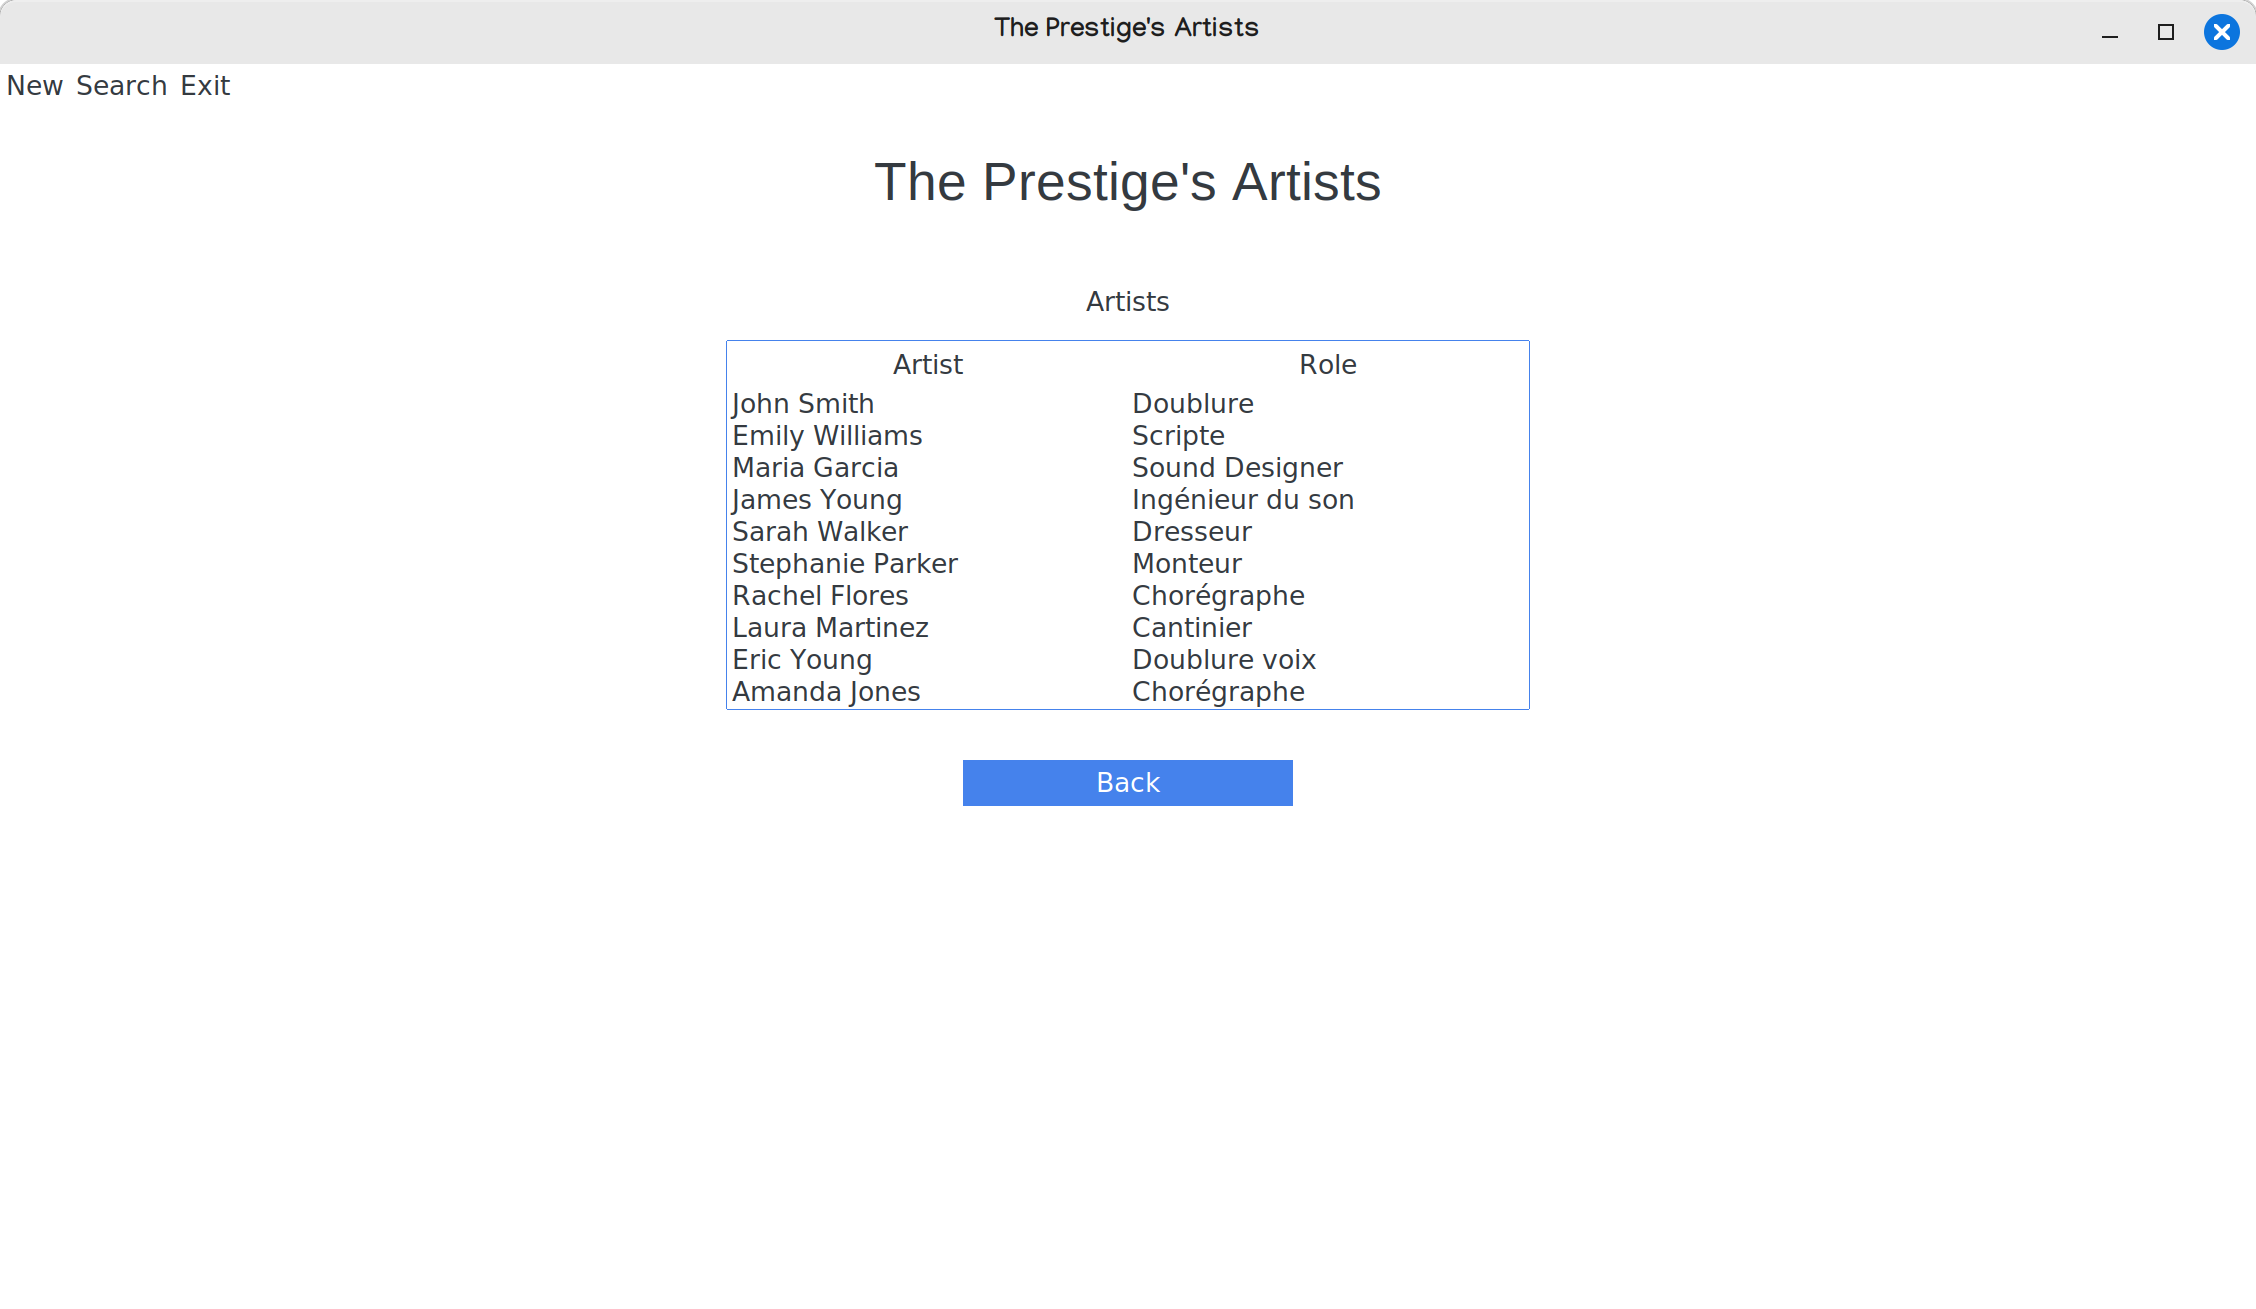
\includegraphics[scale=0.16]{castingartist.png}
\end{center}

\subsection{Page de visualisation des pièces de théâtre et des films}

\begin{center}
  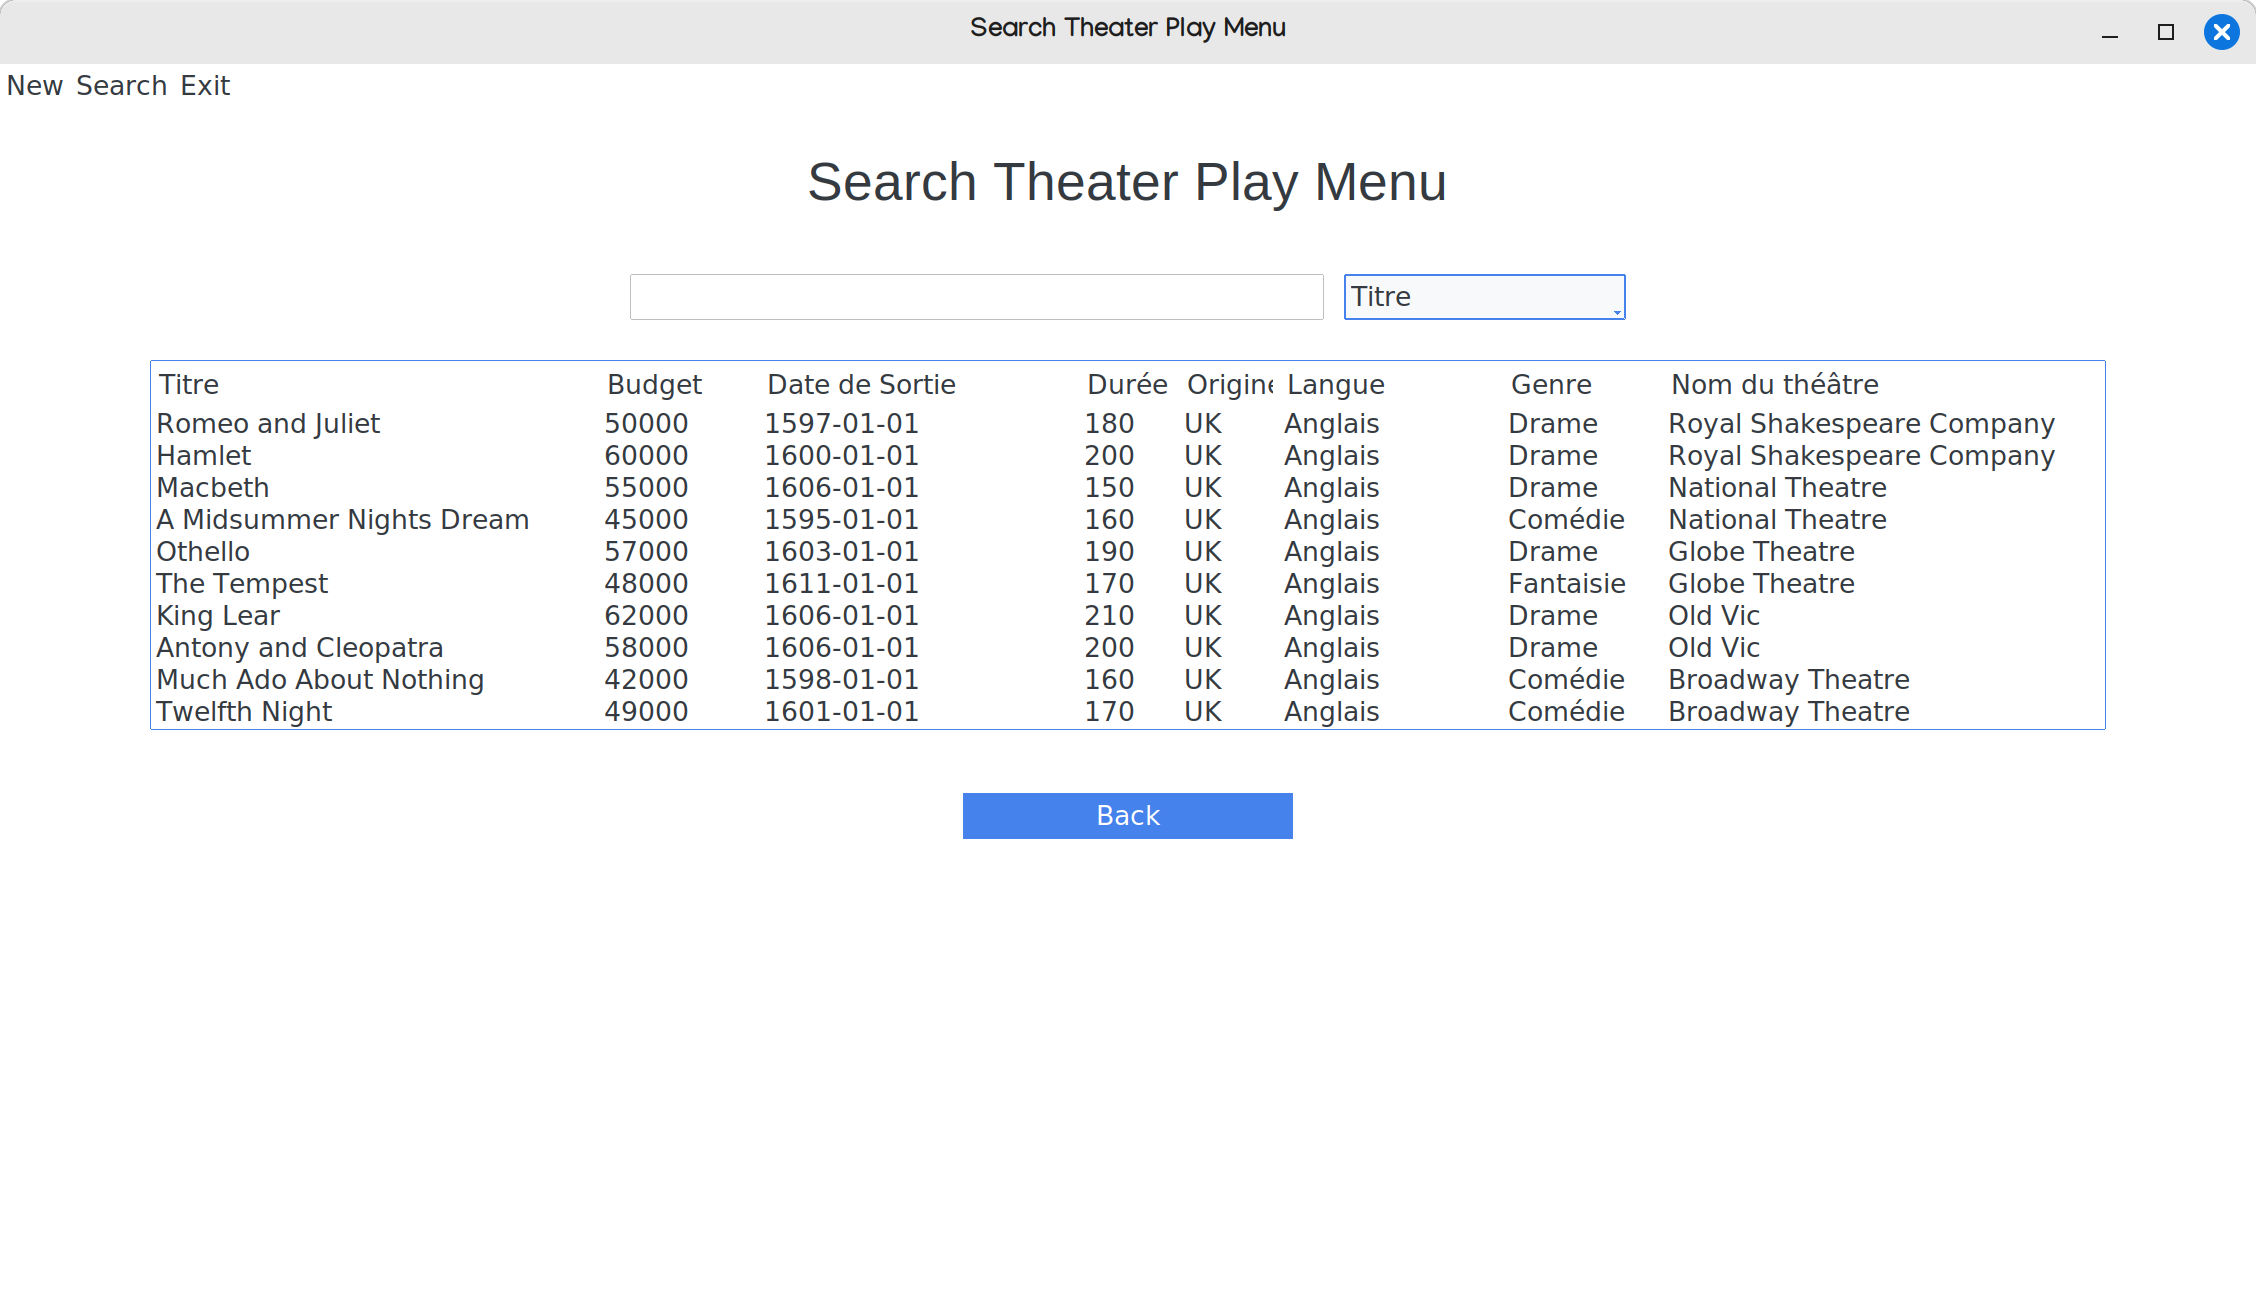
\includegraphics[scale=0.16]{searchplay.png}\n
  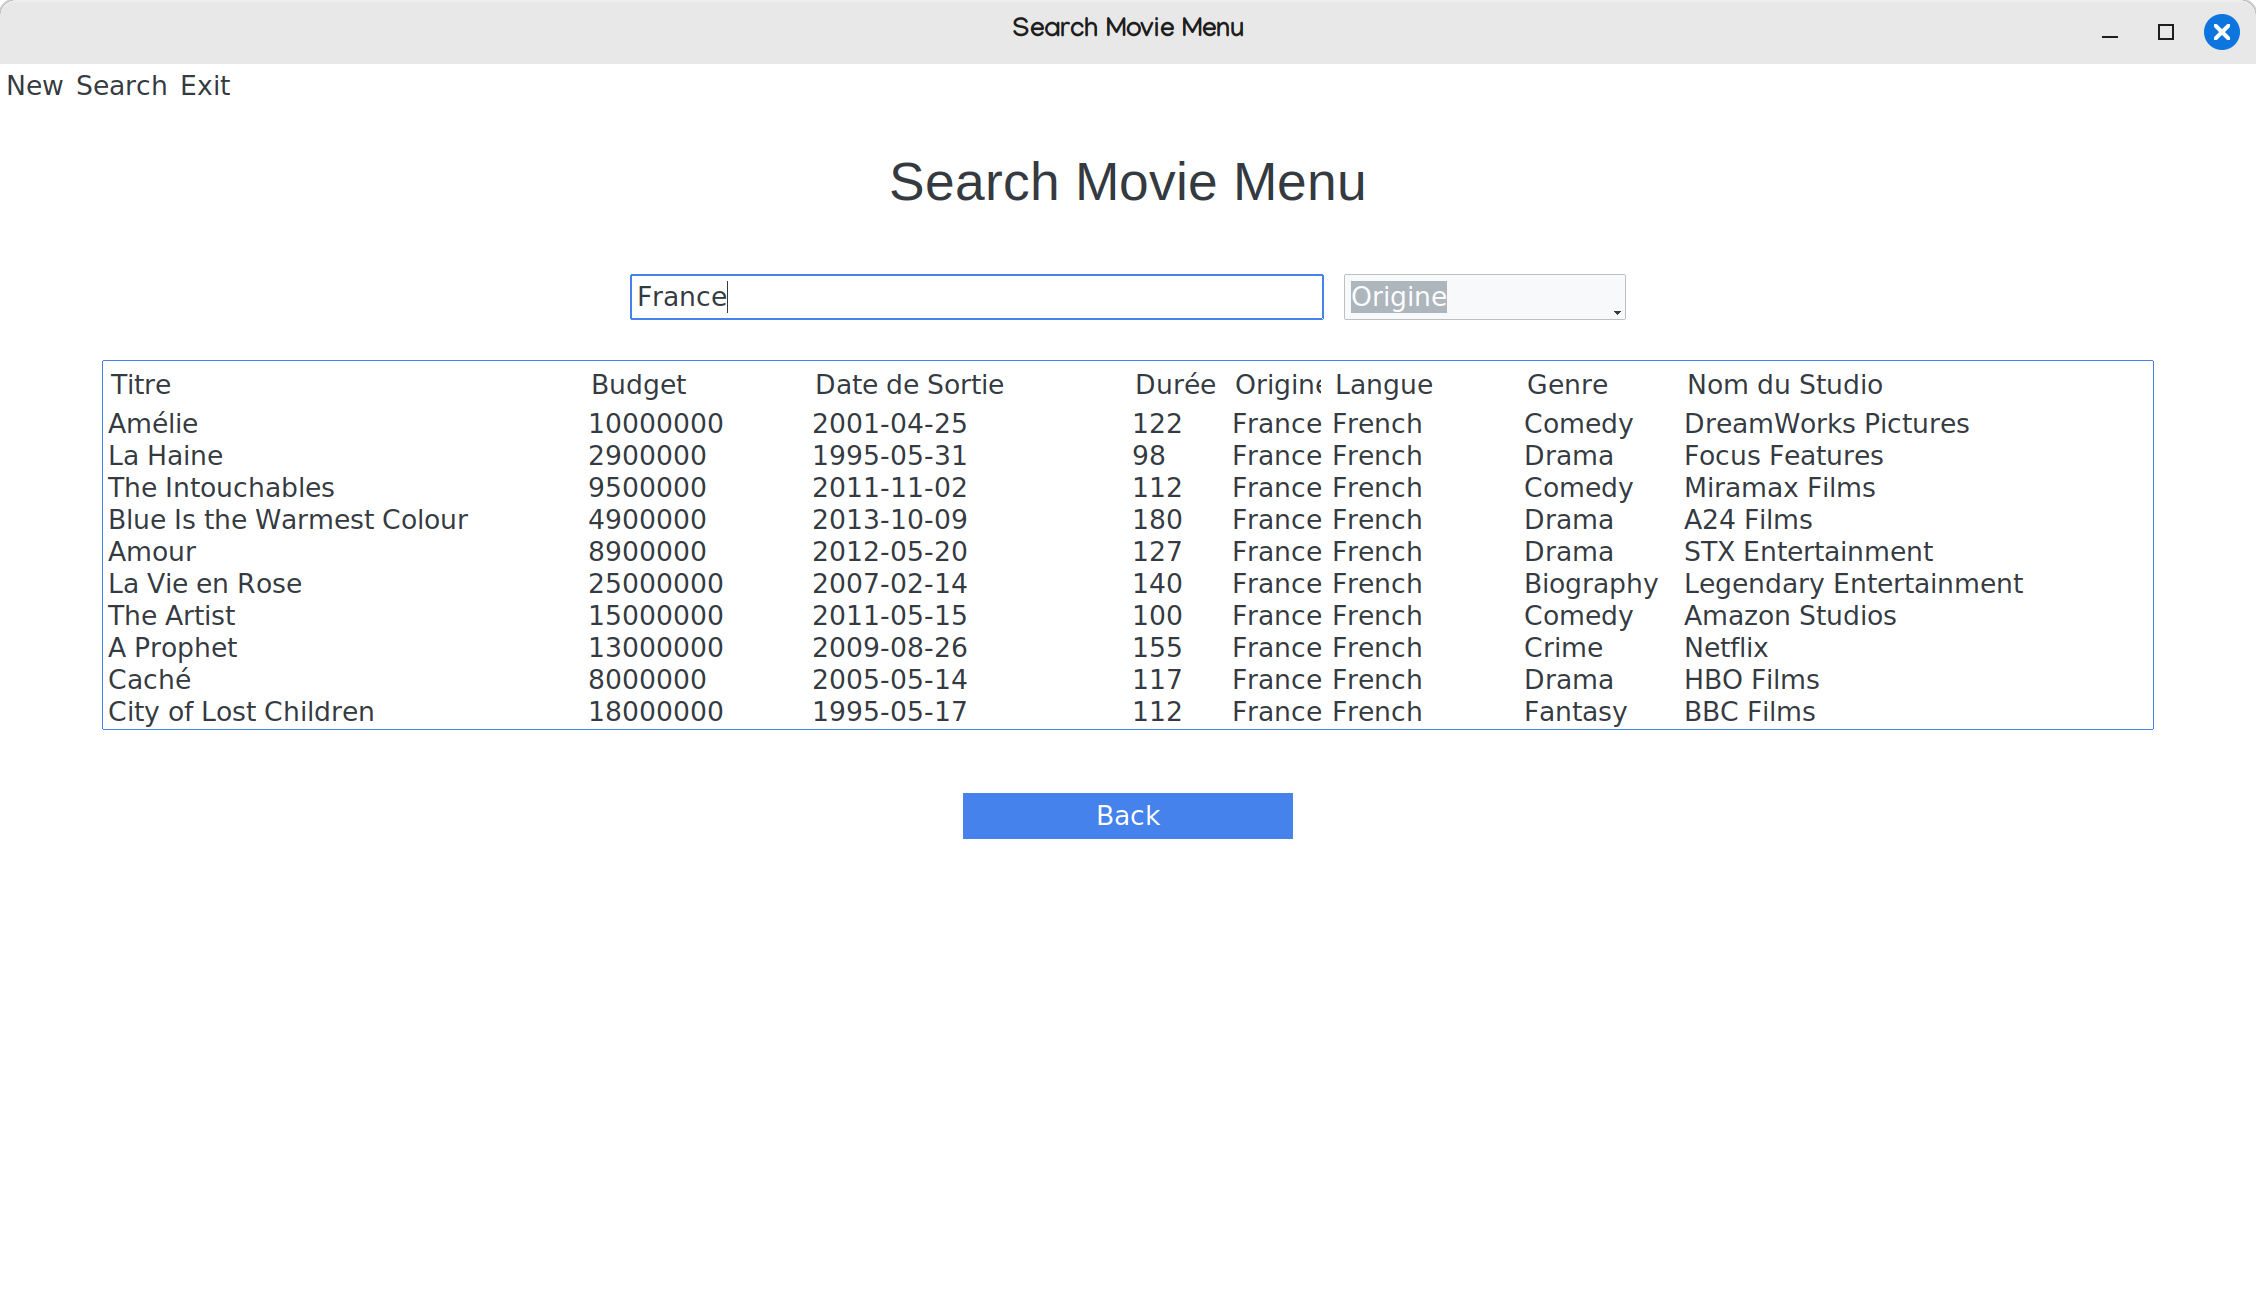
\includegraphics[scale=0.16]{searchmovies1.png}\n
  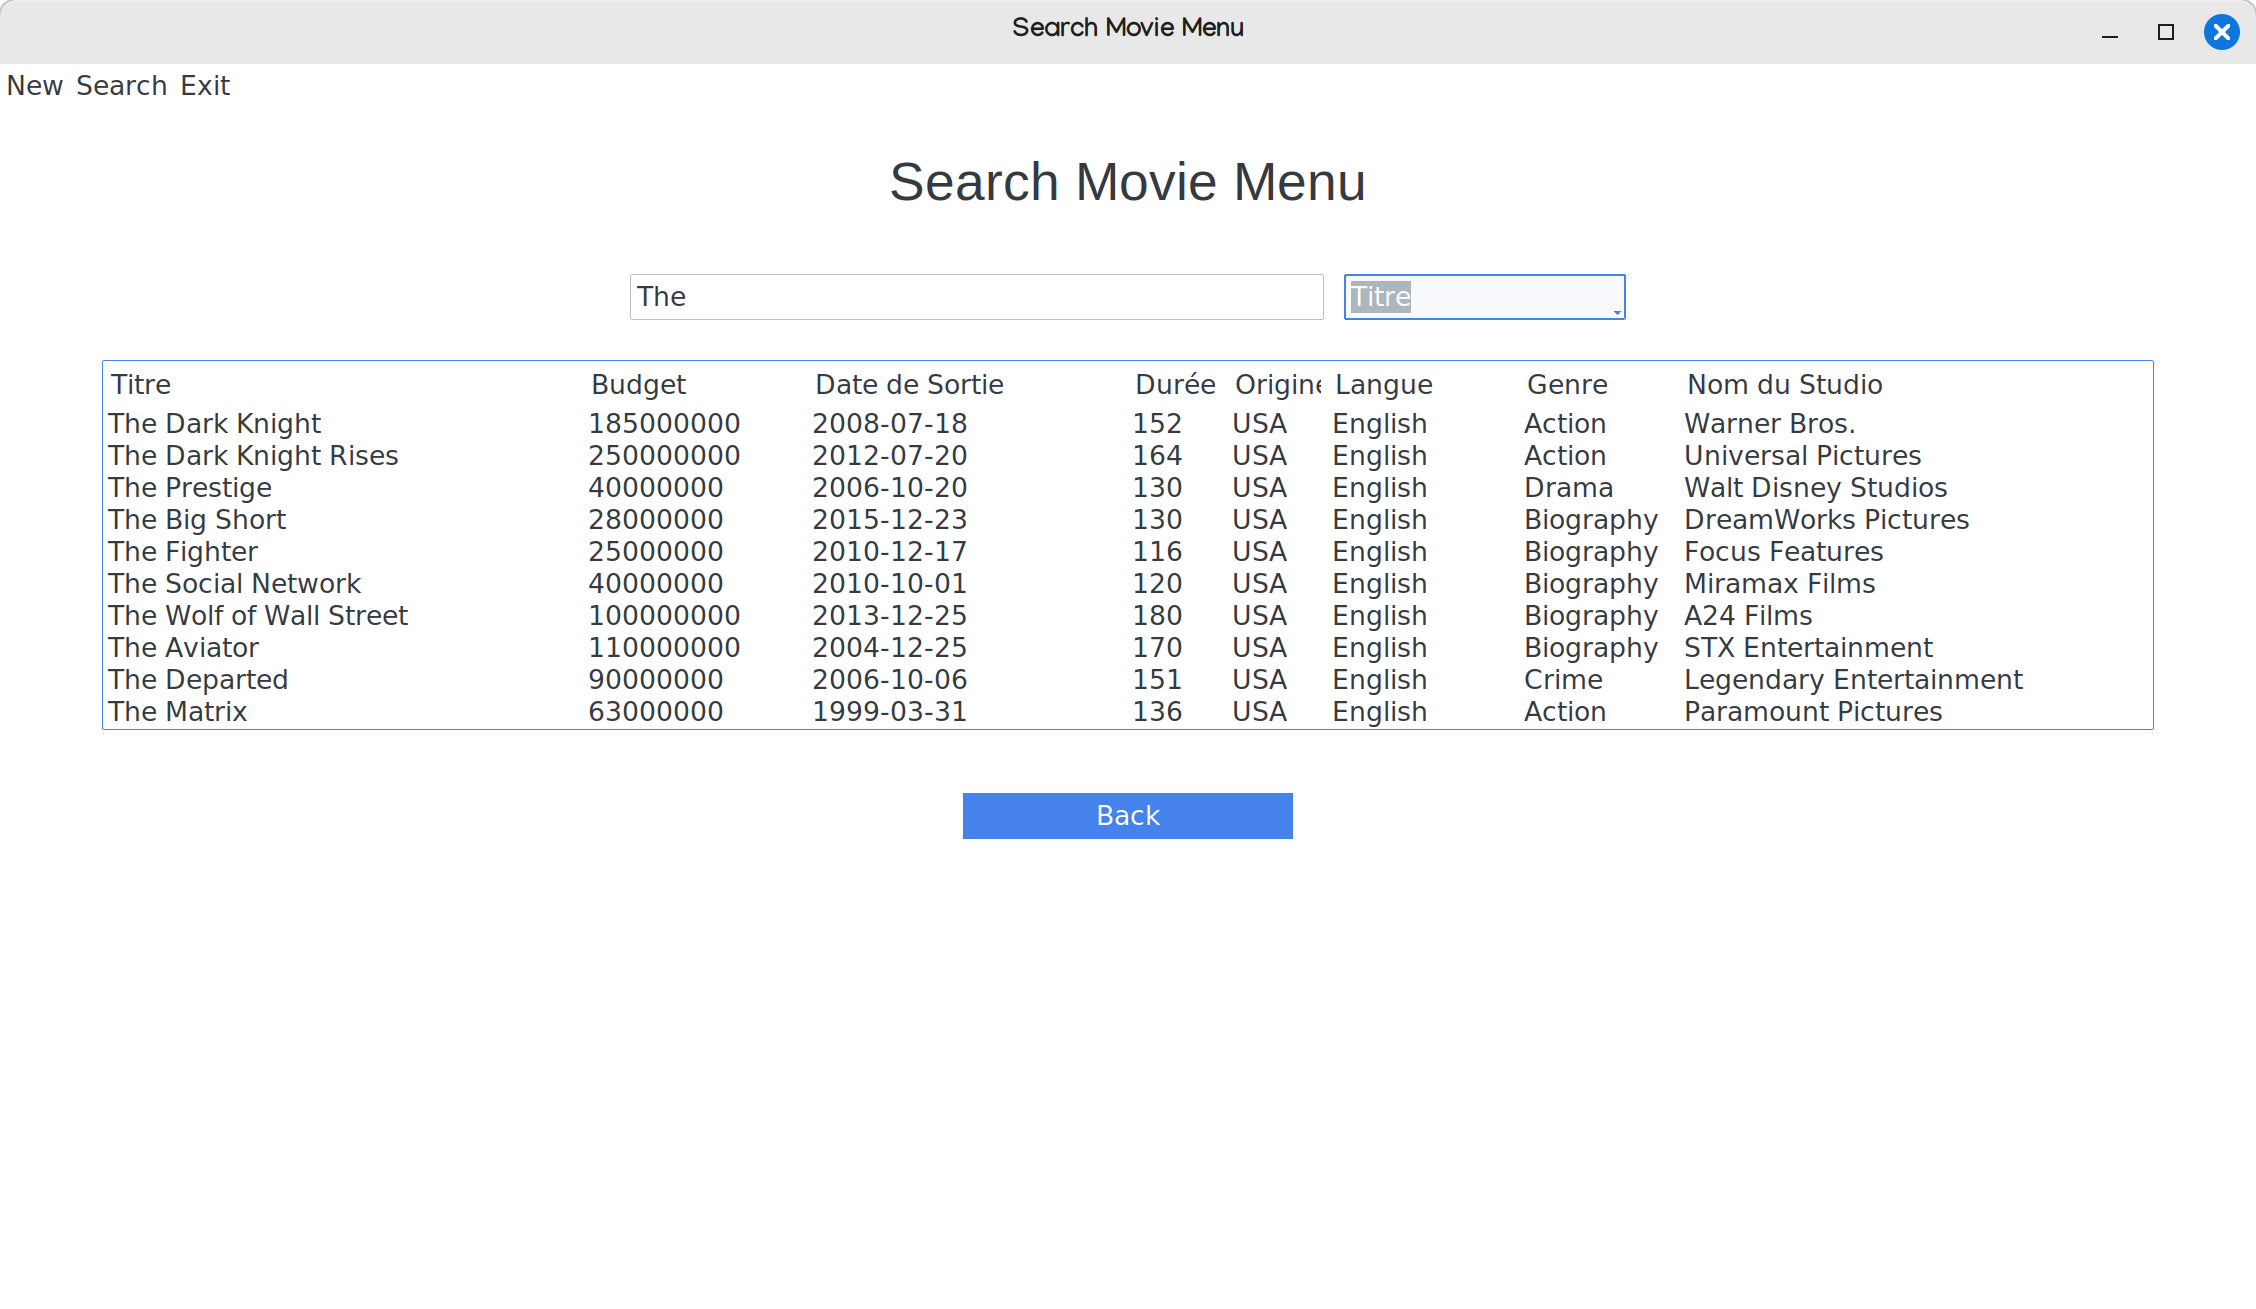
\includegraphics[scale=0.16]{searchmovies2.png}
\end{center}

\newpage

\subsection{Page d'ajout de données}

\begin{center}
 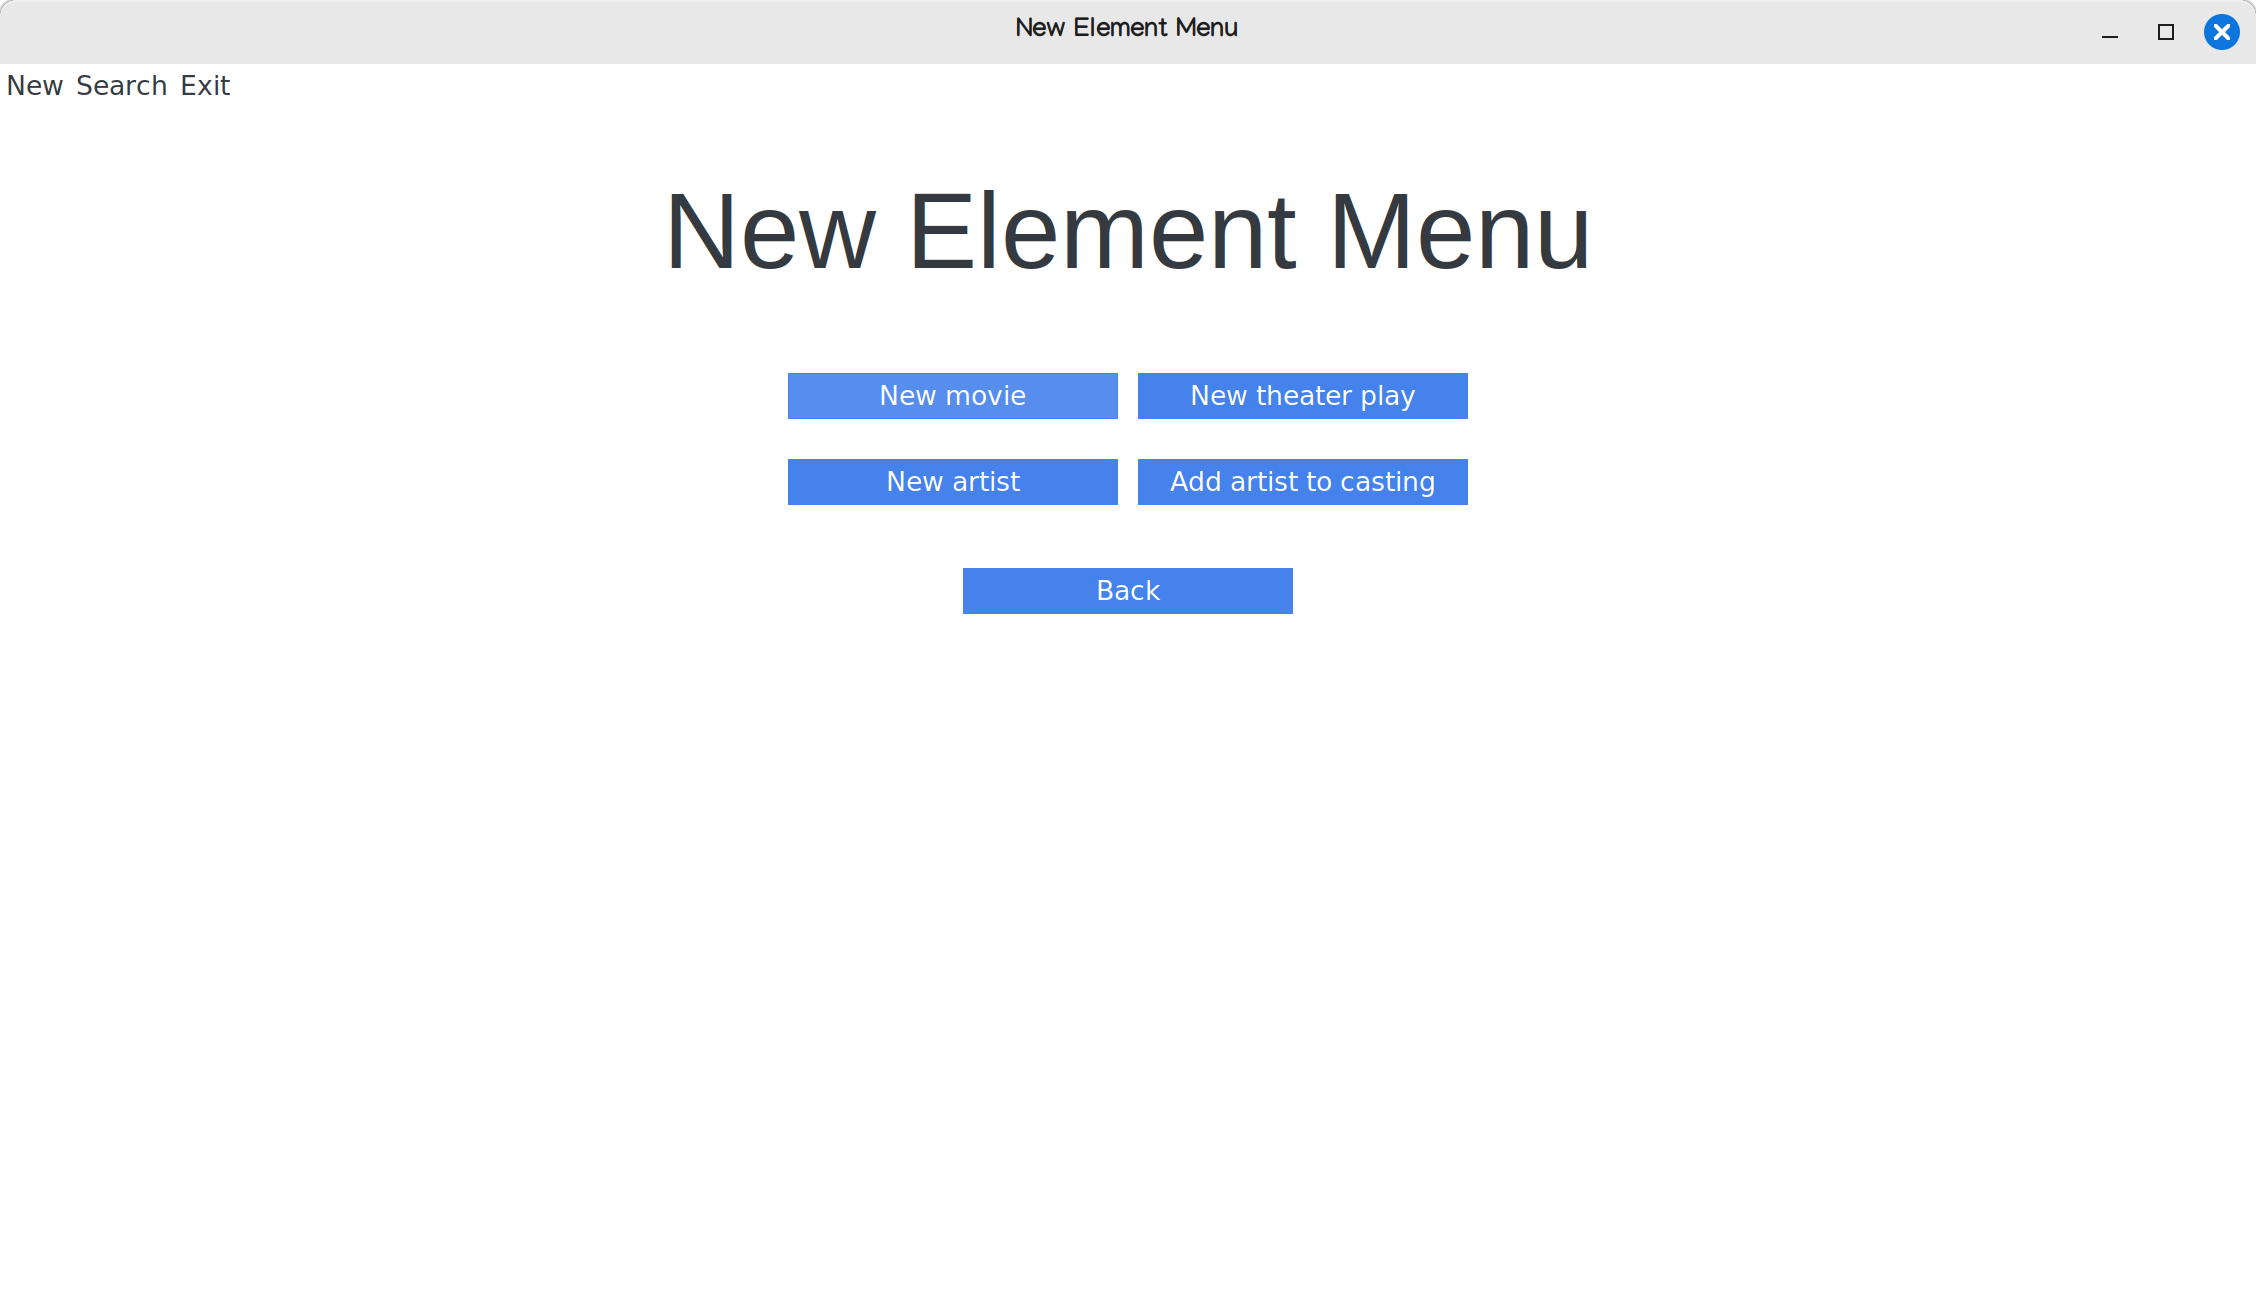
\includegraphics[scale=0.16]{add.png}
\end{center}

\subsection{Page d'ajout d'artiste}

\begin{center}
  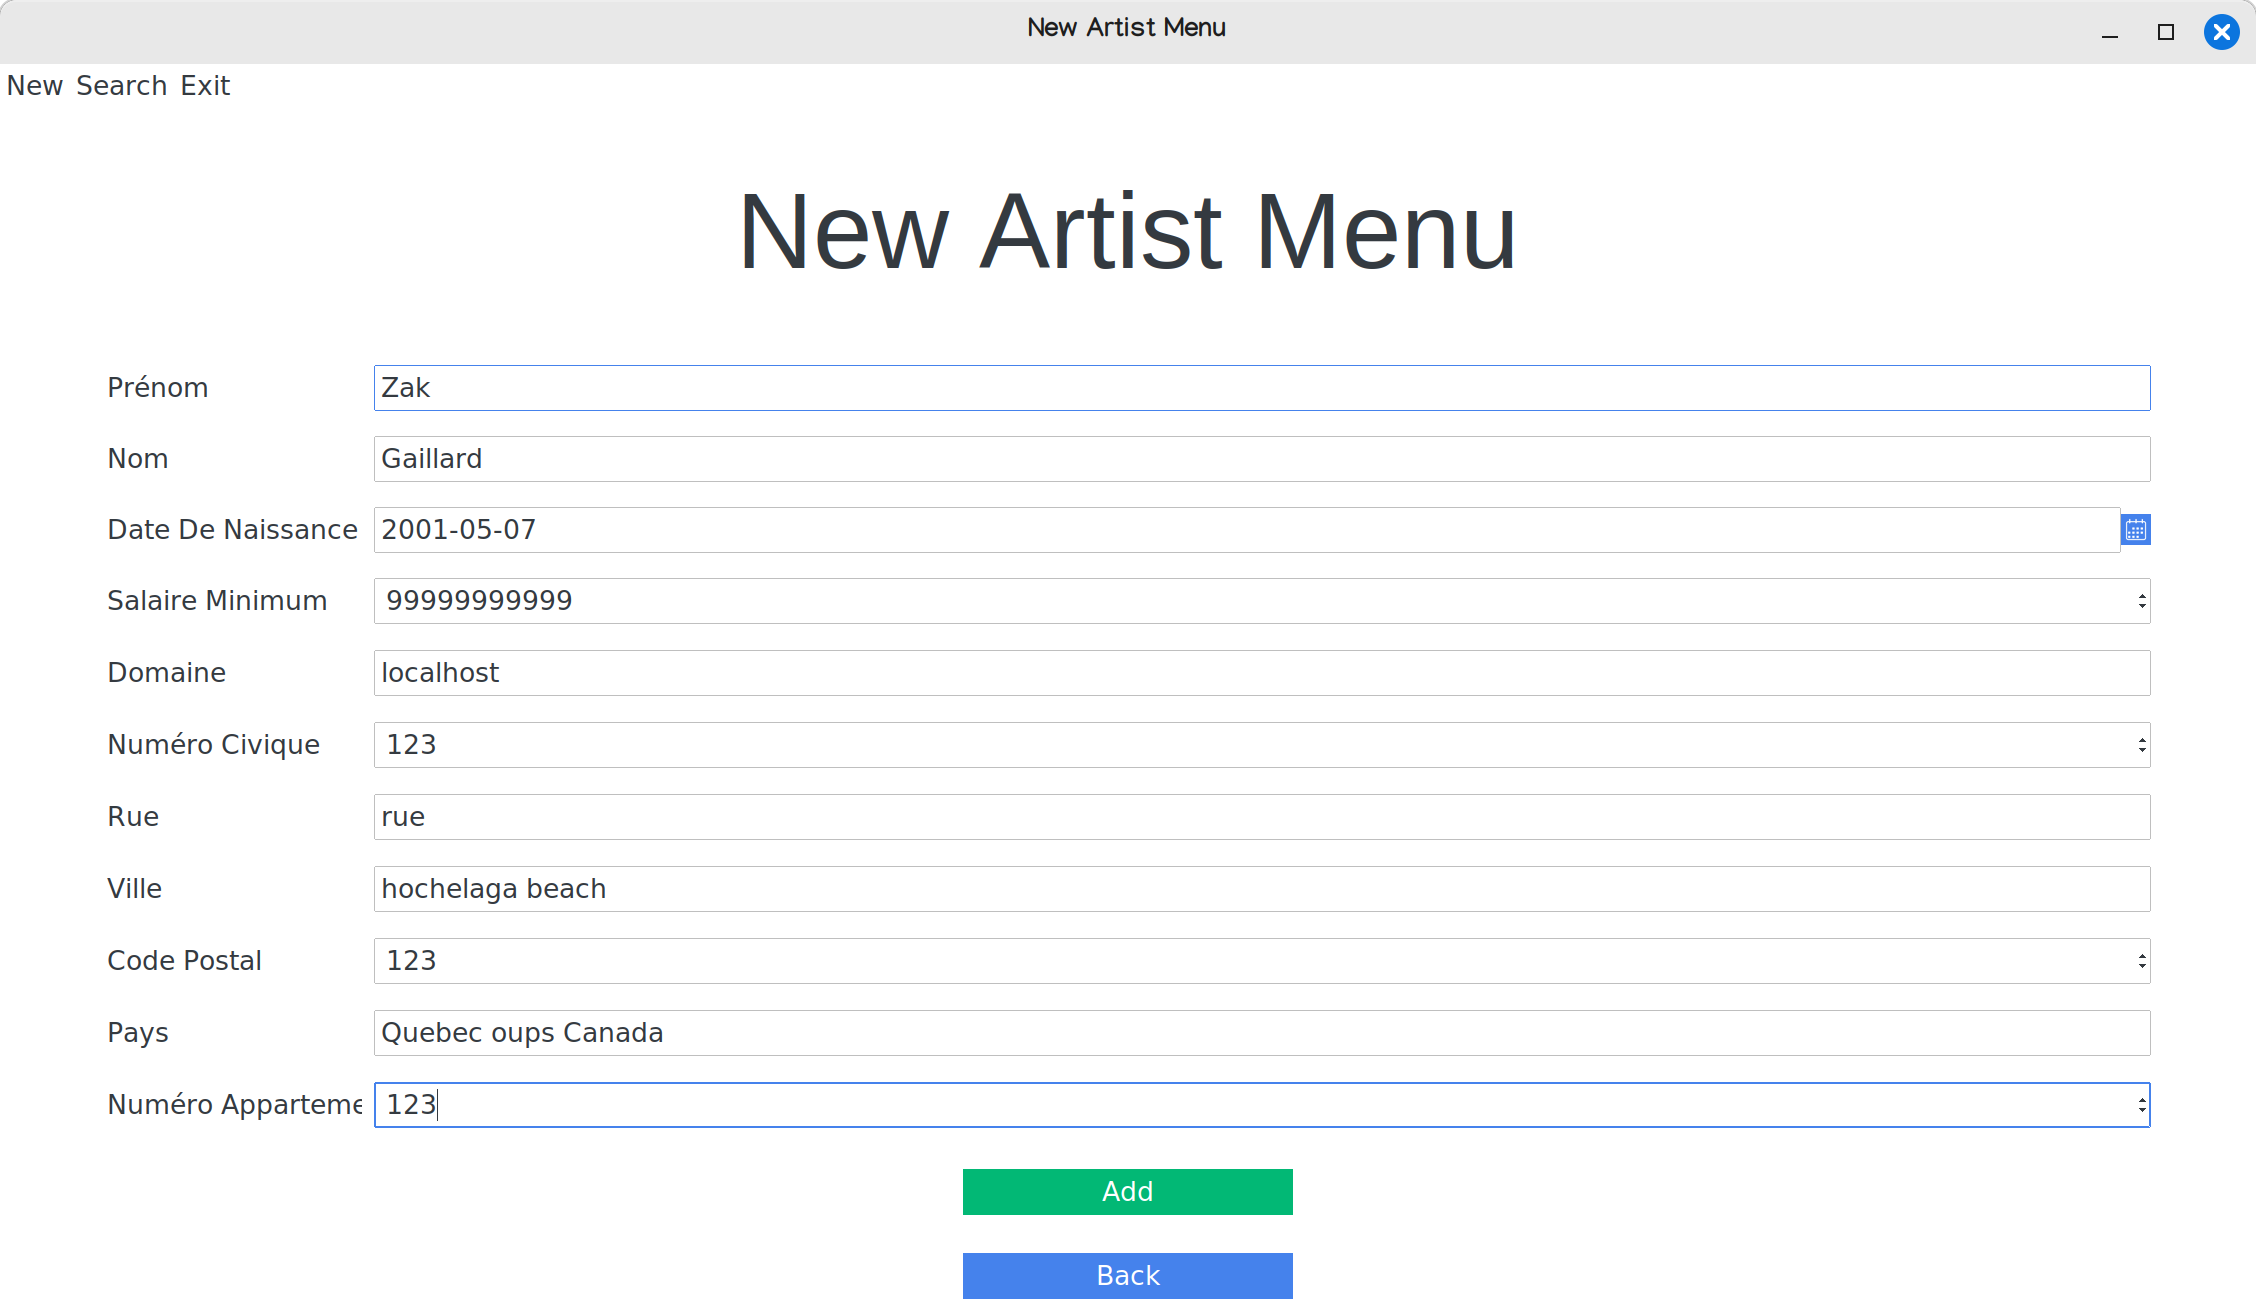
\includegraphics[scale=0.16]{addartist.png}
\end{center}

\subsection{Page d'ajout de pièce de théâtre ou de film}

\begin{center}
  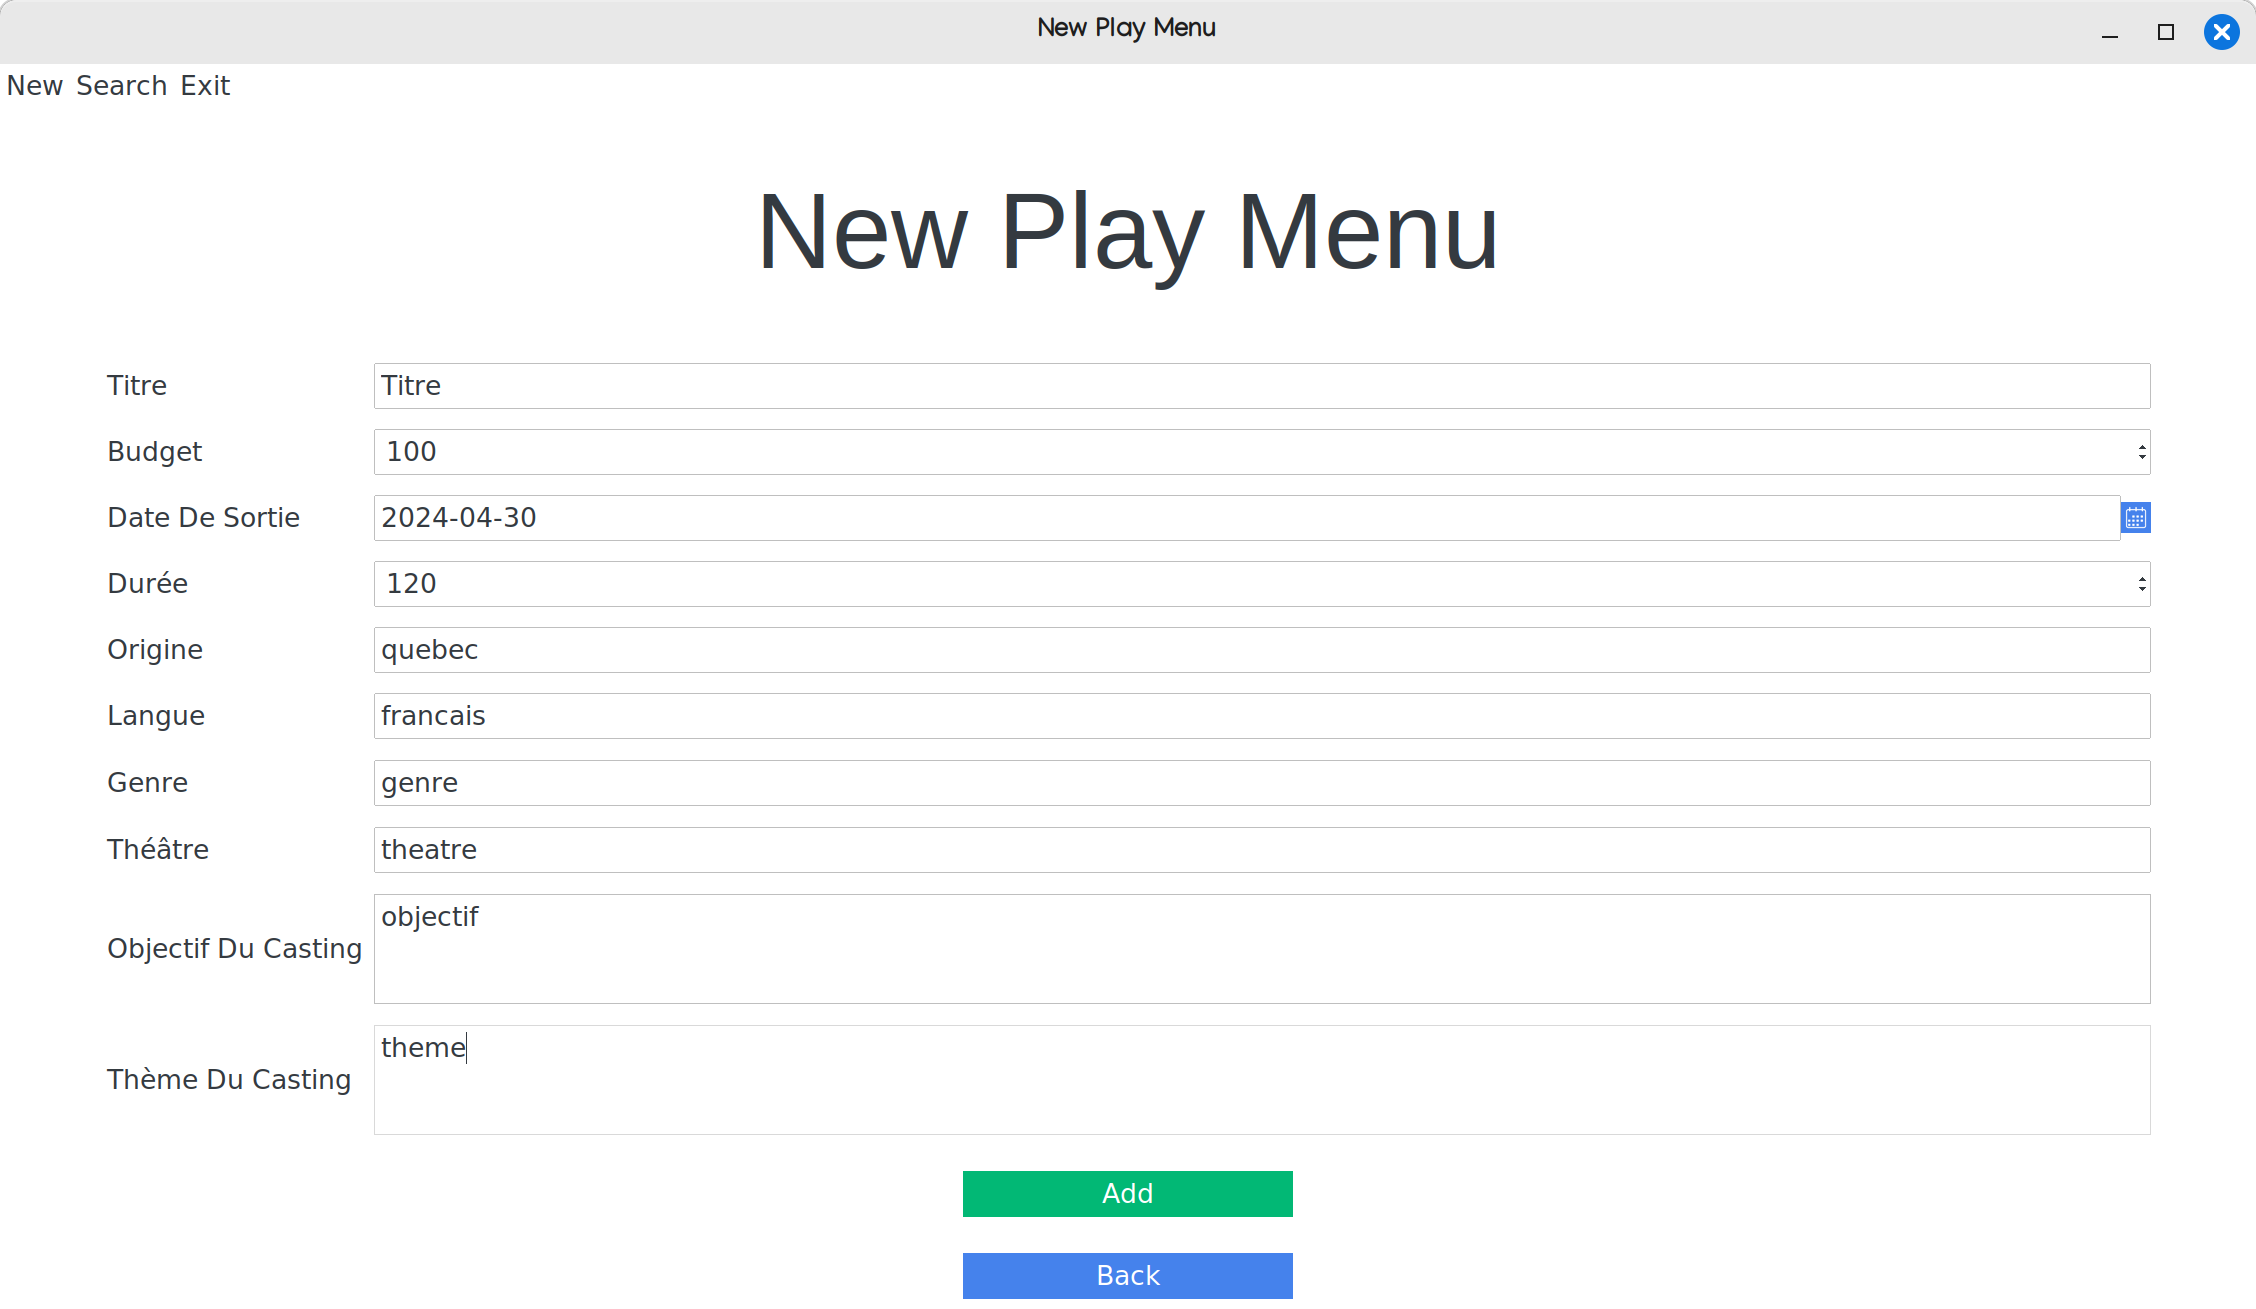
\includegraphics[scale=0.16]{addplay.png}
\end{center}


\subsection{Page d'ajout d'artiste à un casting}

\begin{center}
  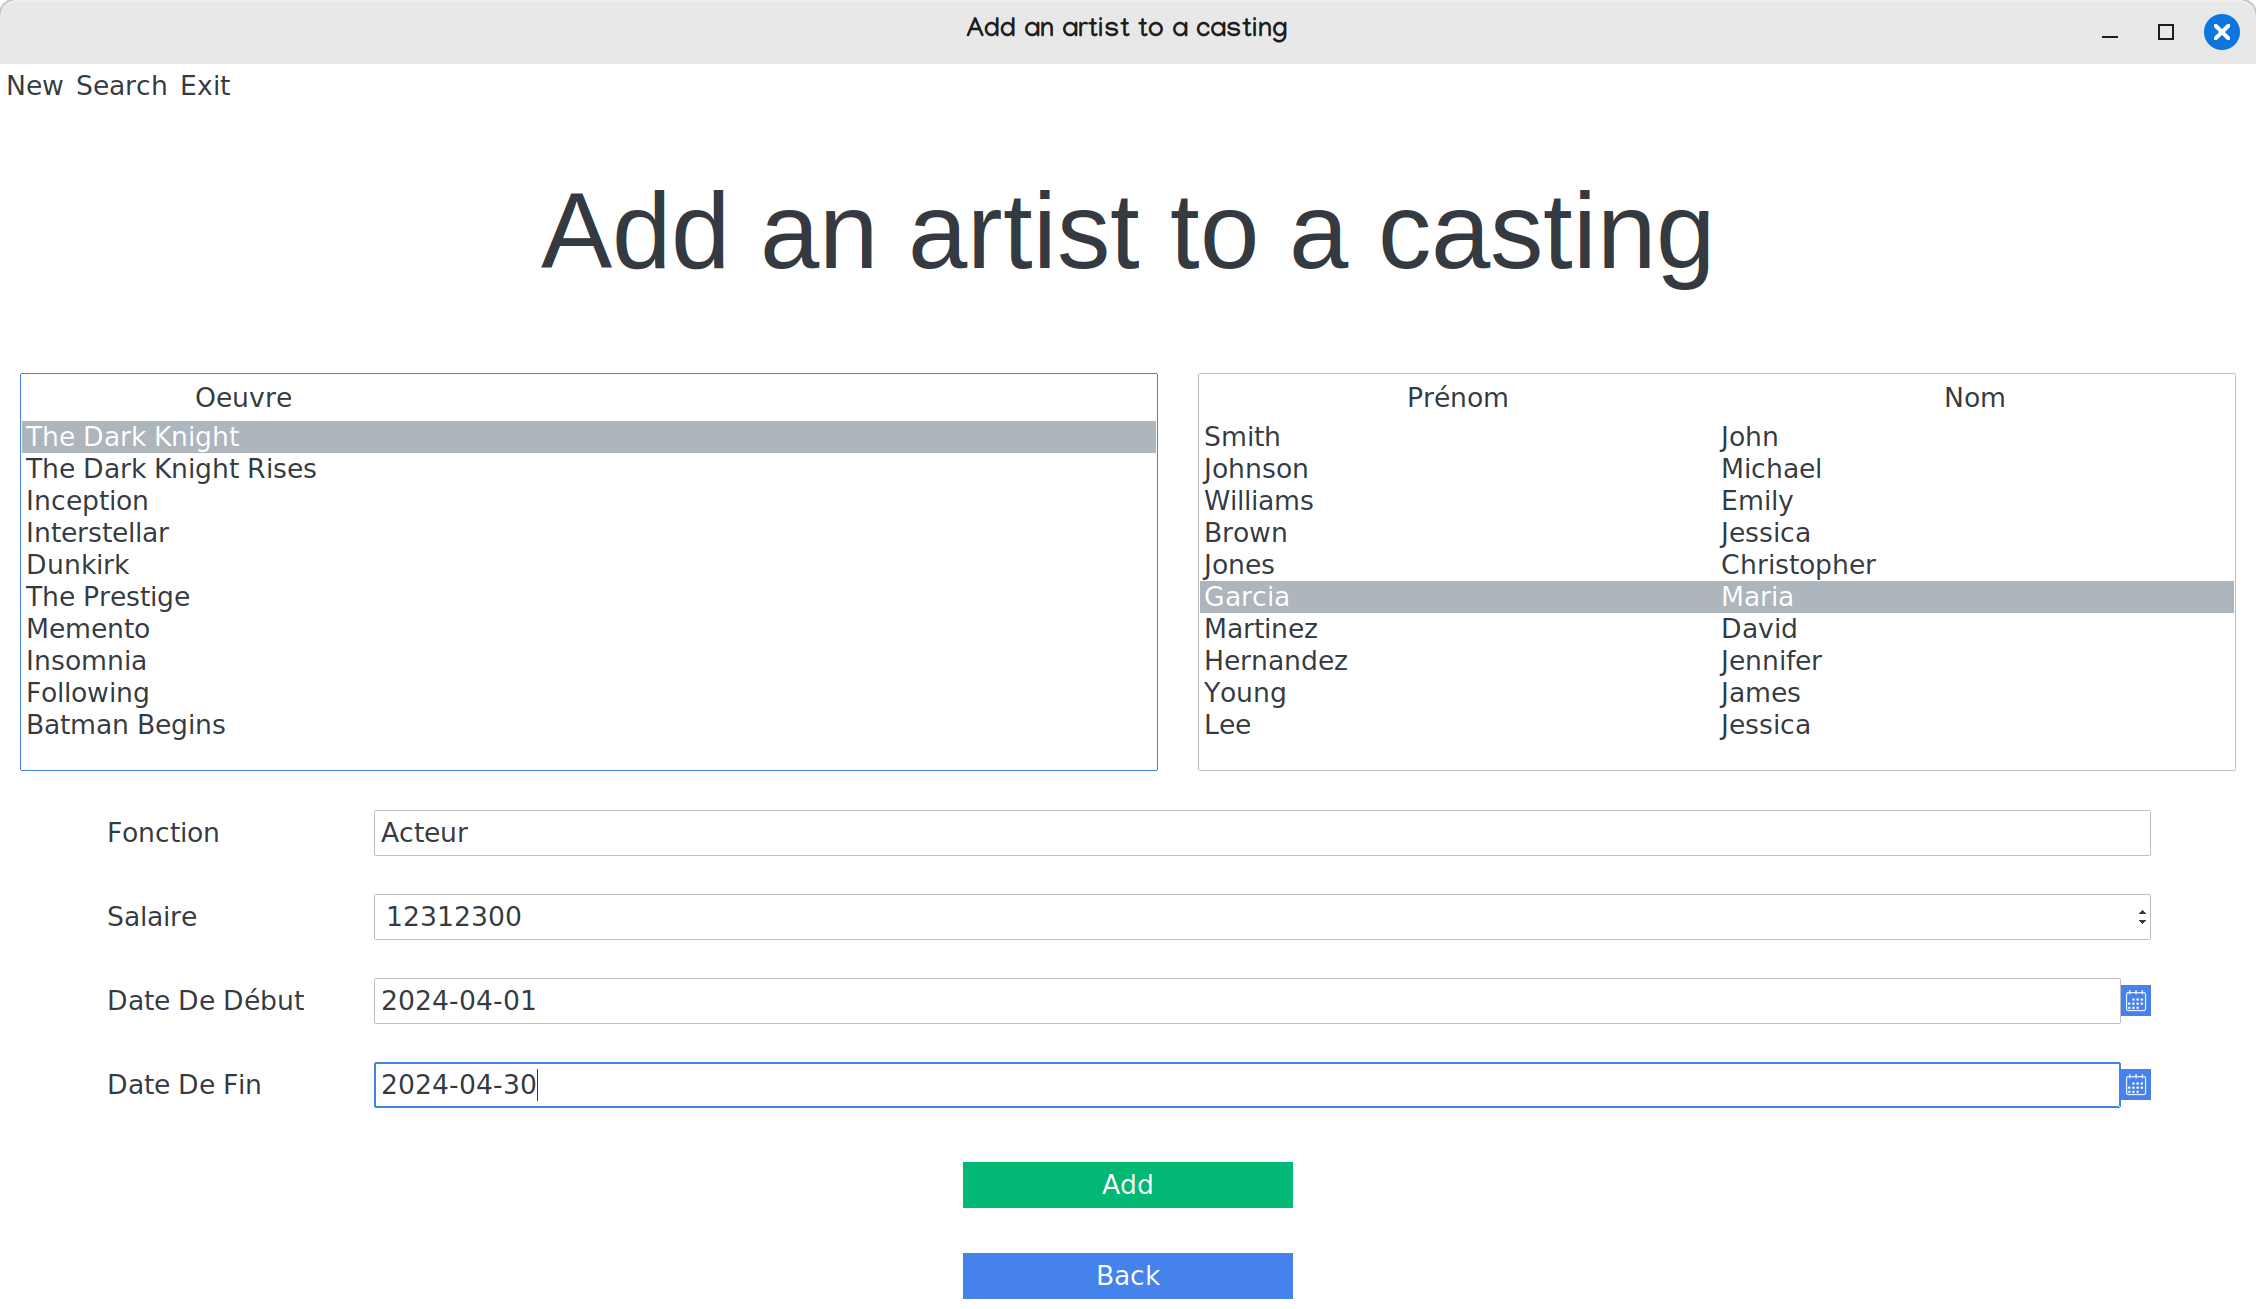
\includegraphics[scale=0.16]{addcasting.png}
\end{center}

\subsection{Message de succès}

\begin{center}
  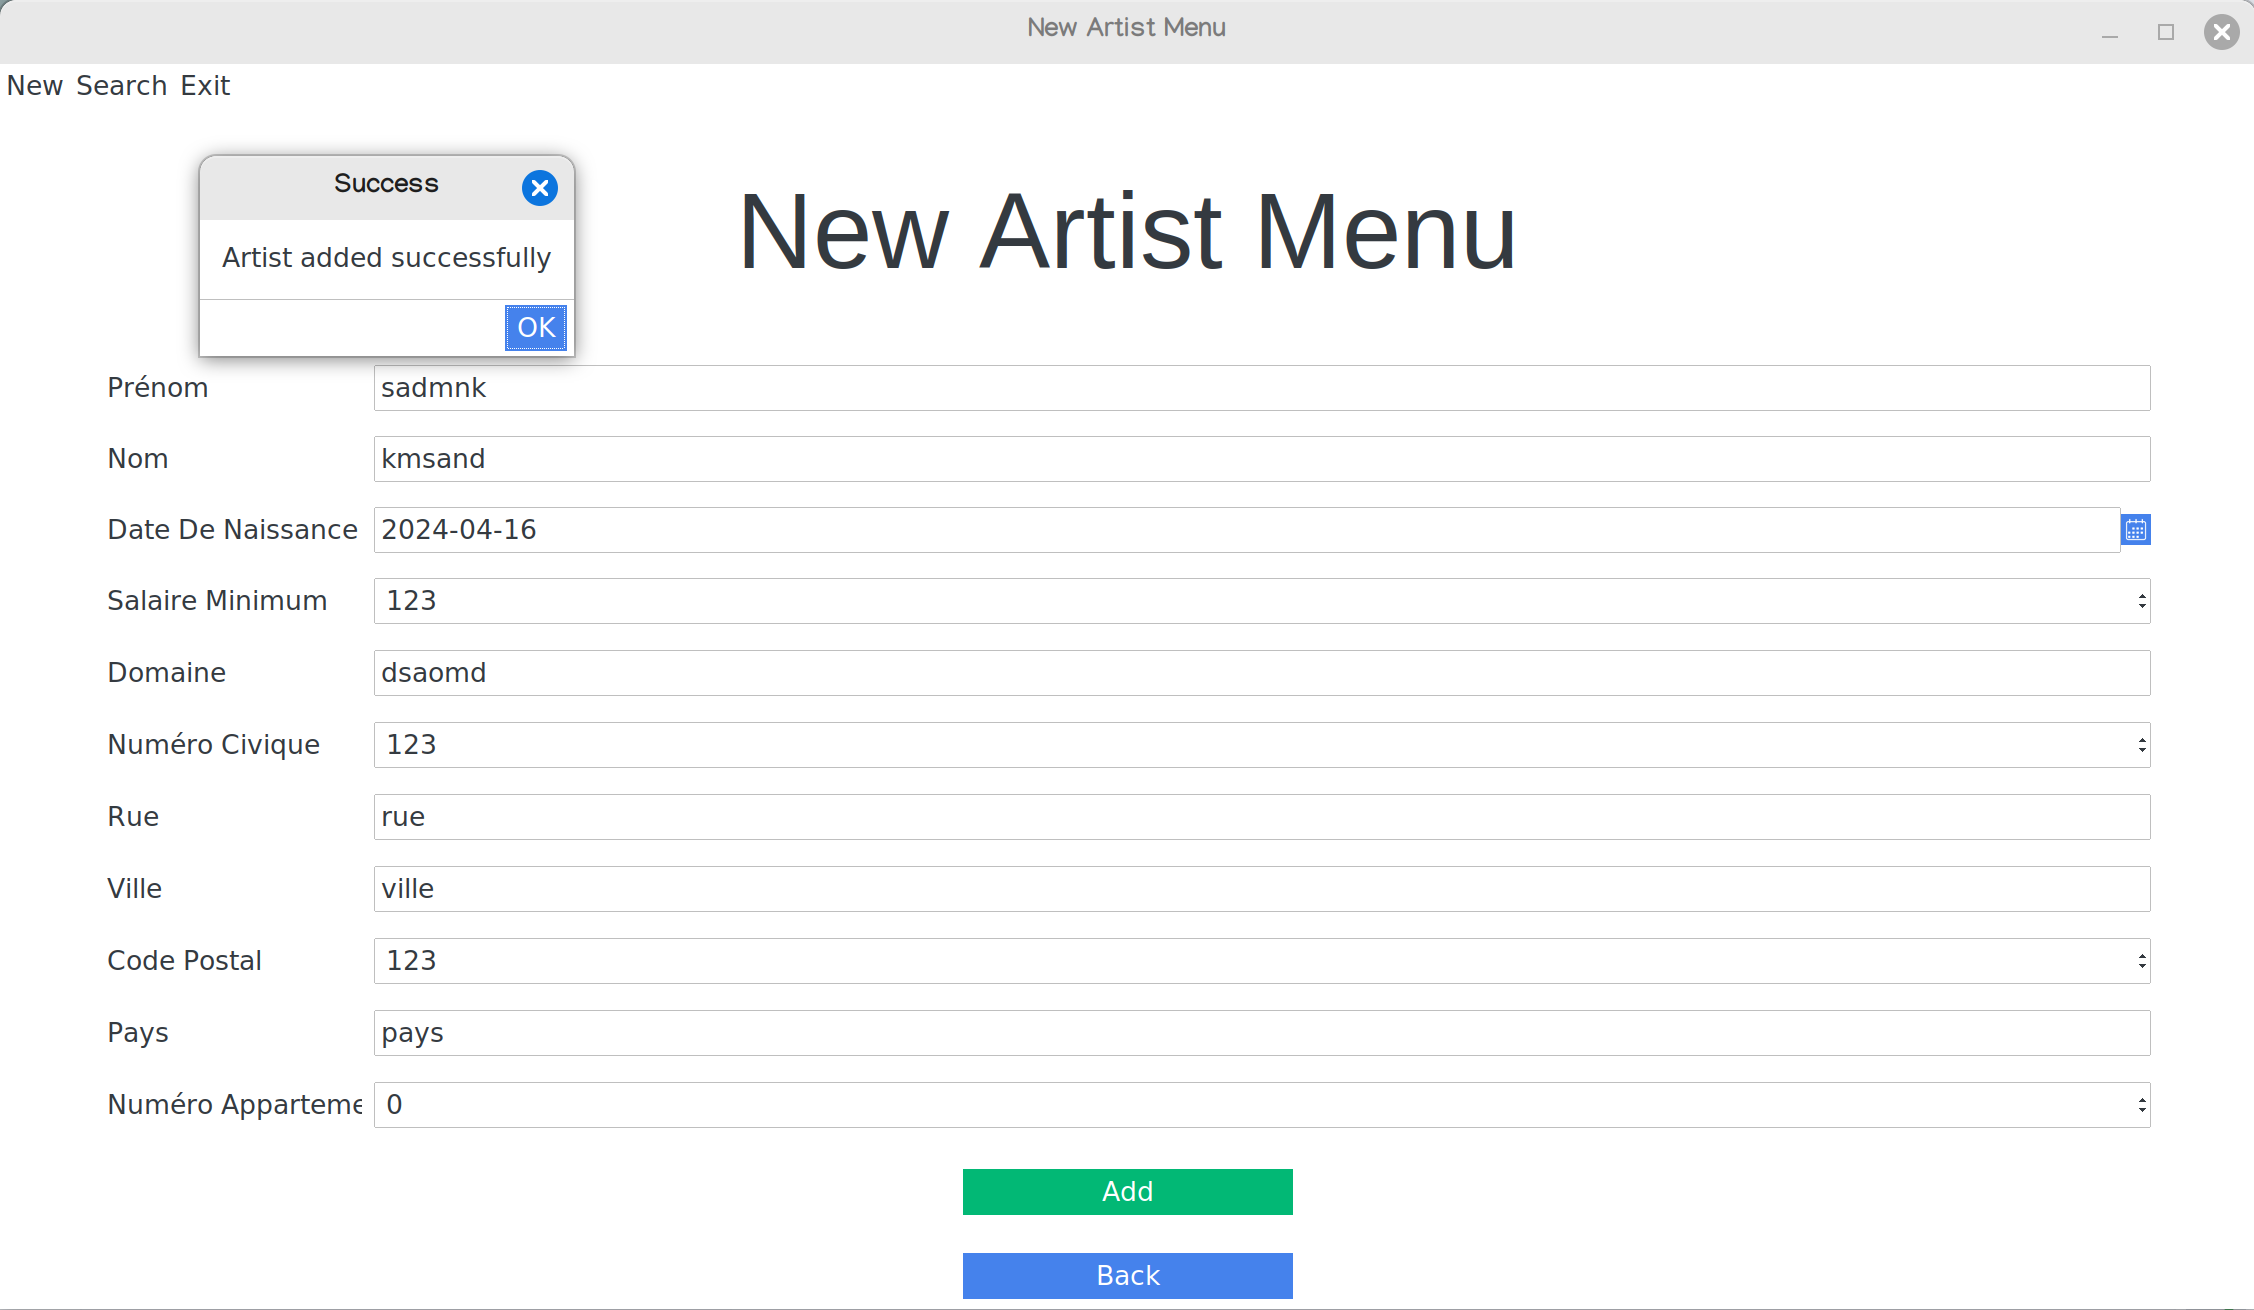
\includegraphics[scale=0.16]{success.png}
\end{center}

\subsection{Message d'erreur}

\begin{center}
   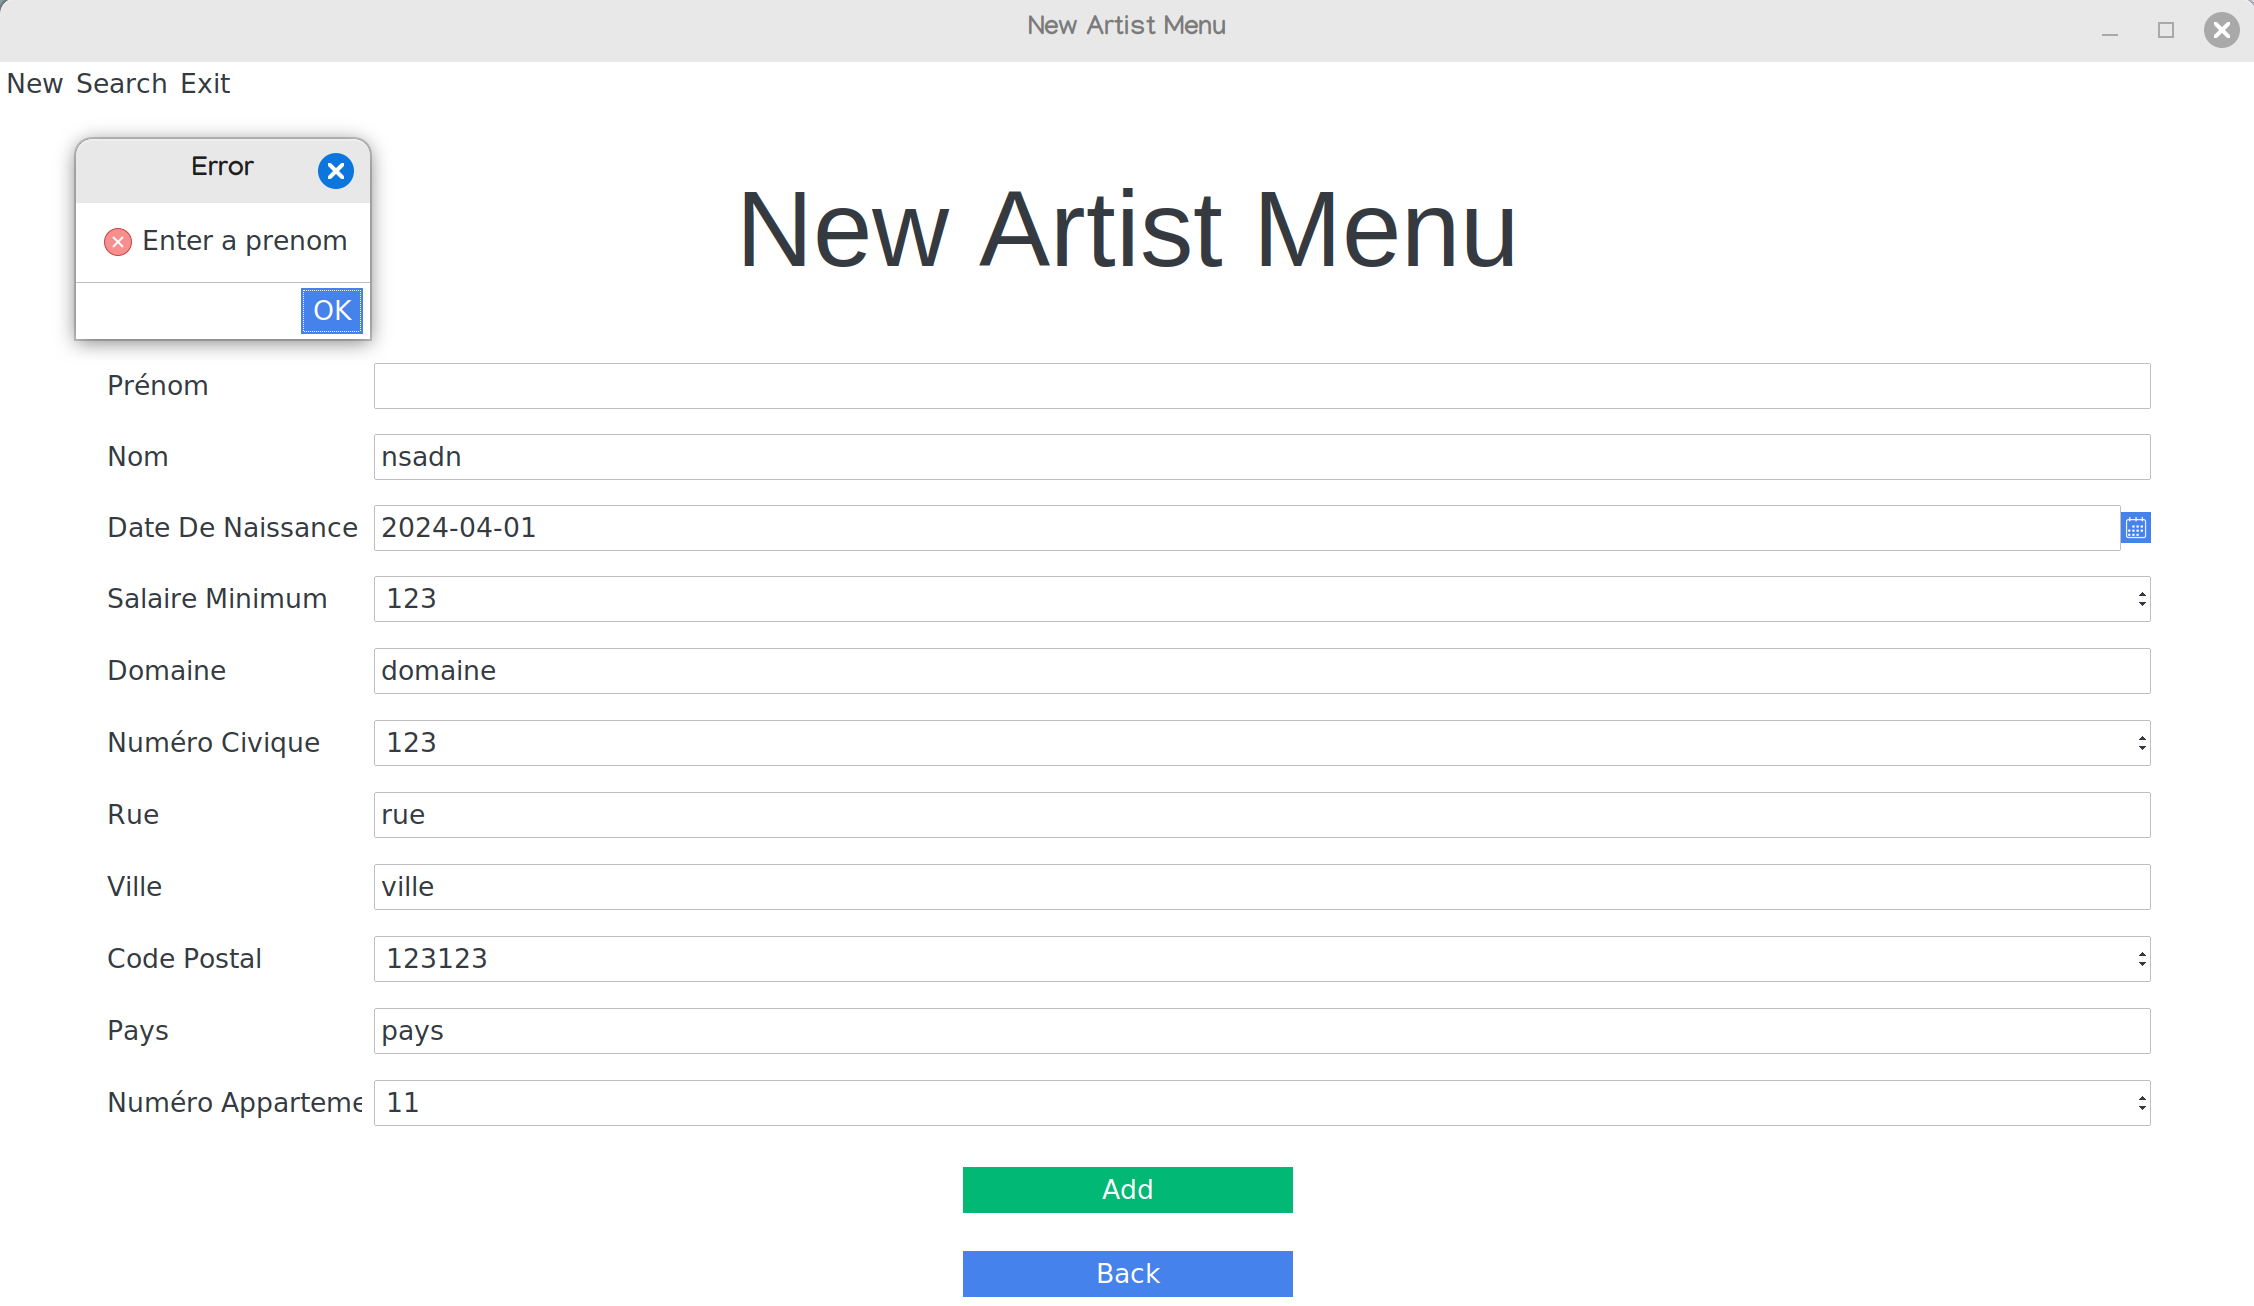
\includegraphics[scale=0.16]{error.png}
\end{center}





  



\end{document}